\documentclass{article}
\usepackage{fancyhdr}
\usepackage{ctex}
\usepackage{listings}
\usepackage{graphicx}
\usepackage[a4paper, body={18cm,22cm}]{geometry}
\usepackage{amsmath,amssymb,amstext,wasysym,enumerate,graphicx}
\usepackage{float,abstract,booktabs,indentfirst,amsmath}
\usepackage{array}
\usepackage{booktabs}
\usepackage{multirow}
\usepackage{url}
\usepackage{diagbox}
\renewcommand\arraystretch{1.4}
\usepackage{indentfirst}
\setlength{\parindent}{2em}
\usepackage{enumitem}
\setmonofont{Consolas}
\usepackage{listings}
\usepackage{xcolor}
\usepackage{makecell}
\usepackage{tikz}
\usetikzlibrary{positioning, arrows.meta}
\setCJKmonofont{黑体}
\lstset{  
	% 基本设置  
	xleftmargin = 3em, xrightmargin = 3em, aboveskip = 1em,  
	backgroundcolor = \color{white},  
	basicstyle = \small\ttfamily,  
	rulesepcolor = \color{gray},  
	breaklines = true,  
	numbers = left,  
	numberstyle = \small,  
	numbersep = -14pt,  
	frame = shadowbox,  
	showspaces = false,  
	columns = fixed,  
	sensitive = true,  
	% VSCode 风格配色  
	keywordstyle = \color{blue!70!black}\bfseries,  
	emphstyle = \color{red!70!black}\bfseries, % 对于强调的词  
	emphstyle=[2]\color{purple!70!black}\bfseries, % 对于第二组强调的词  
	commentstyle = \color{green!60!black}, % 注释颜色  
	stringstyle = \color{orange!90!black}, % 字符串颜色更亮一些  
	morekeywords={ASSERT, int64\_t, uint32\_t},  
	moreemph={ASSERT, NULL},  
	moreemph=[2]{int64\_t, uint32\_t, tid\_t, uint8\_t, int16\_t, uint16\_t, int32\_t, size\_t, bool},  
	morecomment=[l][\color{green!60!black}]{+}, % 以+开头的注释  
}

%--------------------页眉--------------------%
\pagestyle{fancy}
\fancyhead[L]{}
\fancyhead[R]{}
\fancyhead[C]{华东师范大学软件工程学院实验报告}
\fancyfoot[C]{-\thepage-}
\renewcommand{\headrulewidth}{1.5pt}
%--------------------标题--------------------%
\begin{document}
\begin{center}
	{\Large{\textbf{\heiti 华东师范大学软件工程学院实验报告}}}
	\begin{table}[H]
		\centering
		\begin{tabular}{p{2cm}p{4cm}<{\centering}p{1cm}p{2cm}p{6cm}<{\centering}}
			课程名称:    & 操作系统实践 & \quad & 指导教师:    & 张民
			\\ \cline{2-2} \cline{5-5}
			姓\qquad 名: & 王海生    & \quad & 学\qquad 号: & 10235101559         \\ \cline{2-2} \cline{5-5}
			实验编号:    & 实验二 & \quad & 实验名称:    & PintOS修改testcase实验
			\\ \cline{2-2} \cline{5-5}
		\end{tabular}
	\end{table}
	
	% 添加新行并居中
	%\vspace{1em} % 可选:添加垂直间距
	\textbf{代码仓库:}\url{https://github.com/Hanson-Wang-chn/ECNU-Operating-System-WHS.git}
\end{center}
\rule{\textwidth}{1pt}
%--------------------正文--------------------%
\section{实验目的}

\begin{enumerate}[noitemsep, label={{\arabic*})}]
  \item 熟悉PintOS源代码结构
  \item 添加hello-world函数并编译输出
  \item 修改批处理文件实现自动化结果测试
  \item 熟悉\texttt{Visual Studio Code}和\texttt{Git}的使用
\end{enumerate}

\normalsize

\section{实验内容与设计思想}

在这次实验中,我们的主要目标是通过动手实践来加深对PintOS操作系统内部结构的理解,并学习如何在这样的系统中添加自己的代码,实现更多功能。

首先,我们需要\textbf{熟悉PintOS的源代码结构},这包括了解各个文件、文件目录的功能以及它们之间的关系。这样可以帮助我们更好地理解整个系统的运作方式。

接下来,我们将尝试向PintOS中\textbf{添加一个\texttt{hello-world}函数}。这不仅需要正确编写代码,还需要知道如何将新功能整合到现有系统中,并确保它能够顺利编译并通过测试。为了验证我们的\texttt{hello-world}函数是否正常工作,我们还需要\textbf{修改批处理文件},使得每次修改代码后都能自动运行测试程序,从而快速得到反馈。

此外,我们还将学习\textbf{如何使用\texttt{Visual Studio Code}作为开发环境,以及如何利用\texttt{Git}进行版本控制}。这些工具能帮助我们更有效地管理代码,也能提高团队合作效率。

\section{使用环境}

\subsection{主机系统配置}

本次实验的主机系统环境如下表所示:

\begin{center}
	\begin{tabular}{| >{\centering\arraybackslash}m{3cm} | >{\centering\arraybackslash}m{7cm} |}    
		\hline  
		\textbf{项目名称} & \textbf{详细信息} \\
		\hline  
		操作系统 & macOS Sequoia 15.0 \\  
		\hline  
		系统类型 & 64位操作系统,基于ARM的处理器 \\  
		\hline
		CPU & Apple M1 Pro \\  
		\hline 
		GPU & Apple M1 Pro\\  
		\hline 
		内存 & 16GB 统一内存 \\  
		\hline 
		磁盘 & 512GB SSD \\  
		\hline 		
	\end{tabular}
\end{center}

\subsection{Docker配置}

在官网下载并安装后,Docker容器正常运行,如下图所示:

\begin{figure}[H]
	\centering
	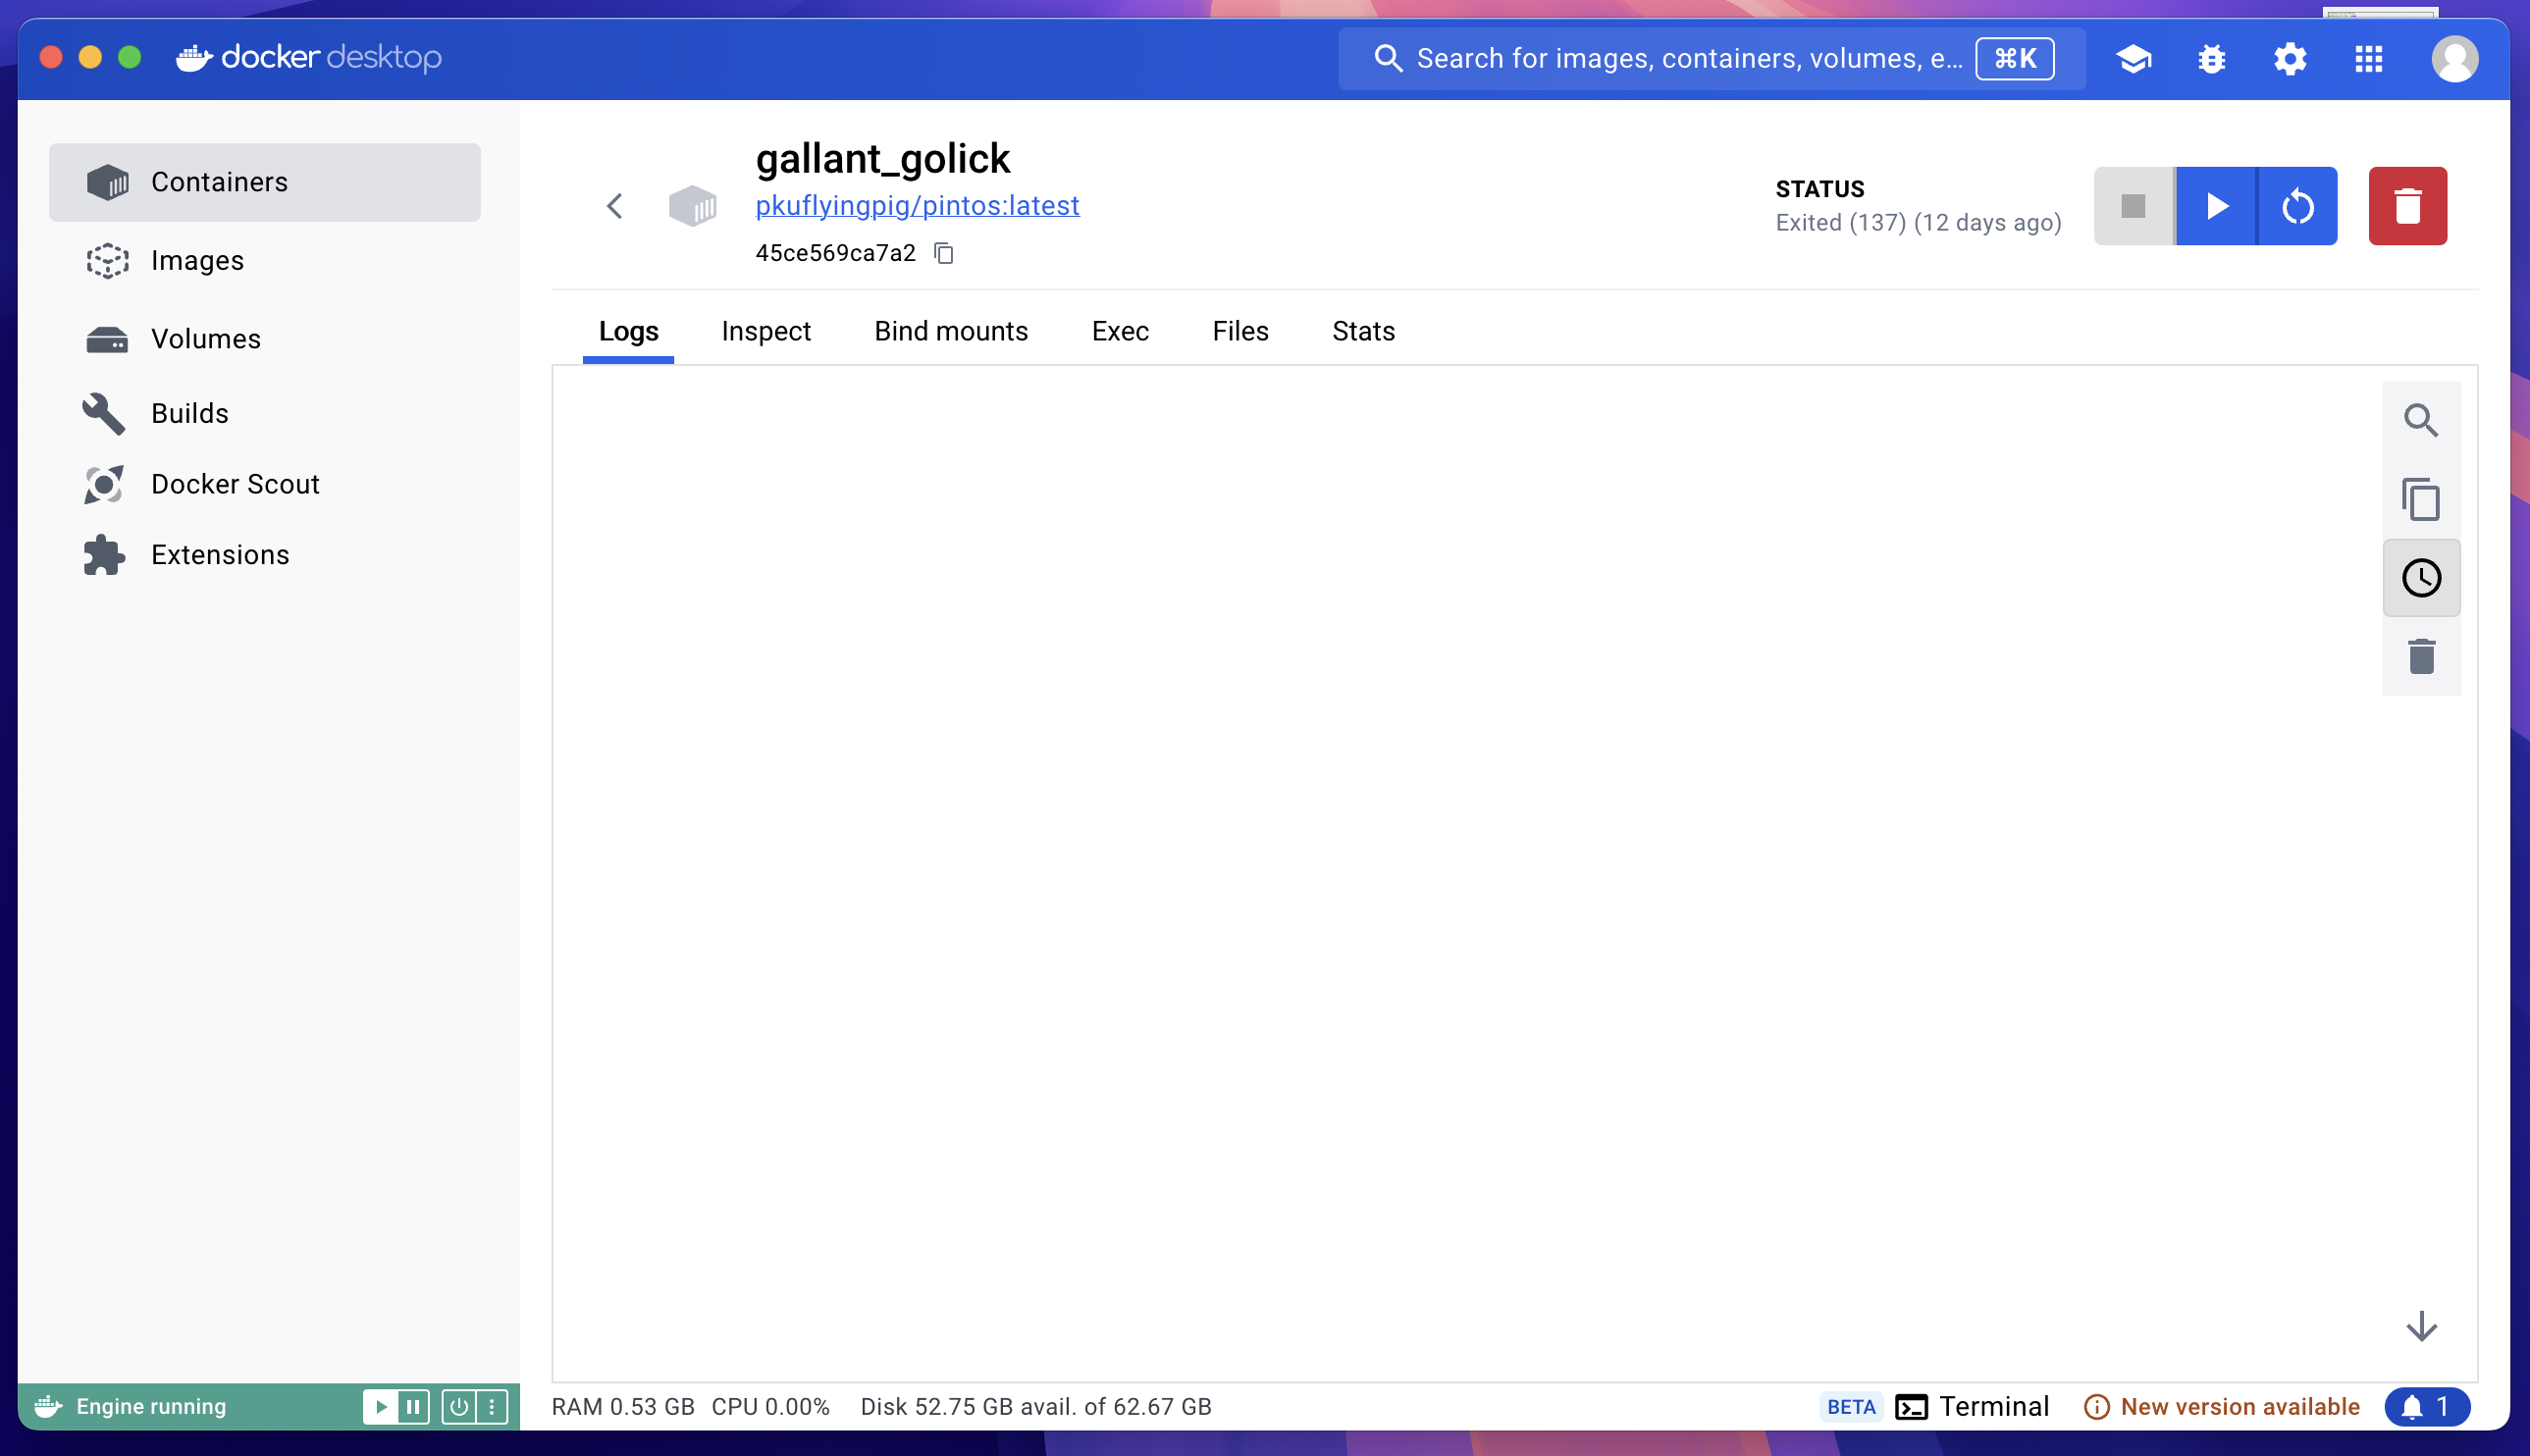
\includegraphics[width=0.9\textwidth]{img/docker_install.png}
	\caption{Docker容器}
\end{figure}

接着使用下面的命令实现磁盘挂载,方便文件管理:

\begin{lstlisting}[language=Bash, title=启动Docker容器并挂载文件]
	docker run -it --rm --name pintos --mount type=bind,\
	source=/Users/wanghaisheng/Desktop/Coding/ECNU-Operating-System-WHS/pintos,\
	target=/home/PKUOS/pintos pkuflyingpig/pintos bash
\end{lstlisting}

完成后如下图所示:

\begin{figure}[H]
	\centering
	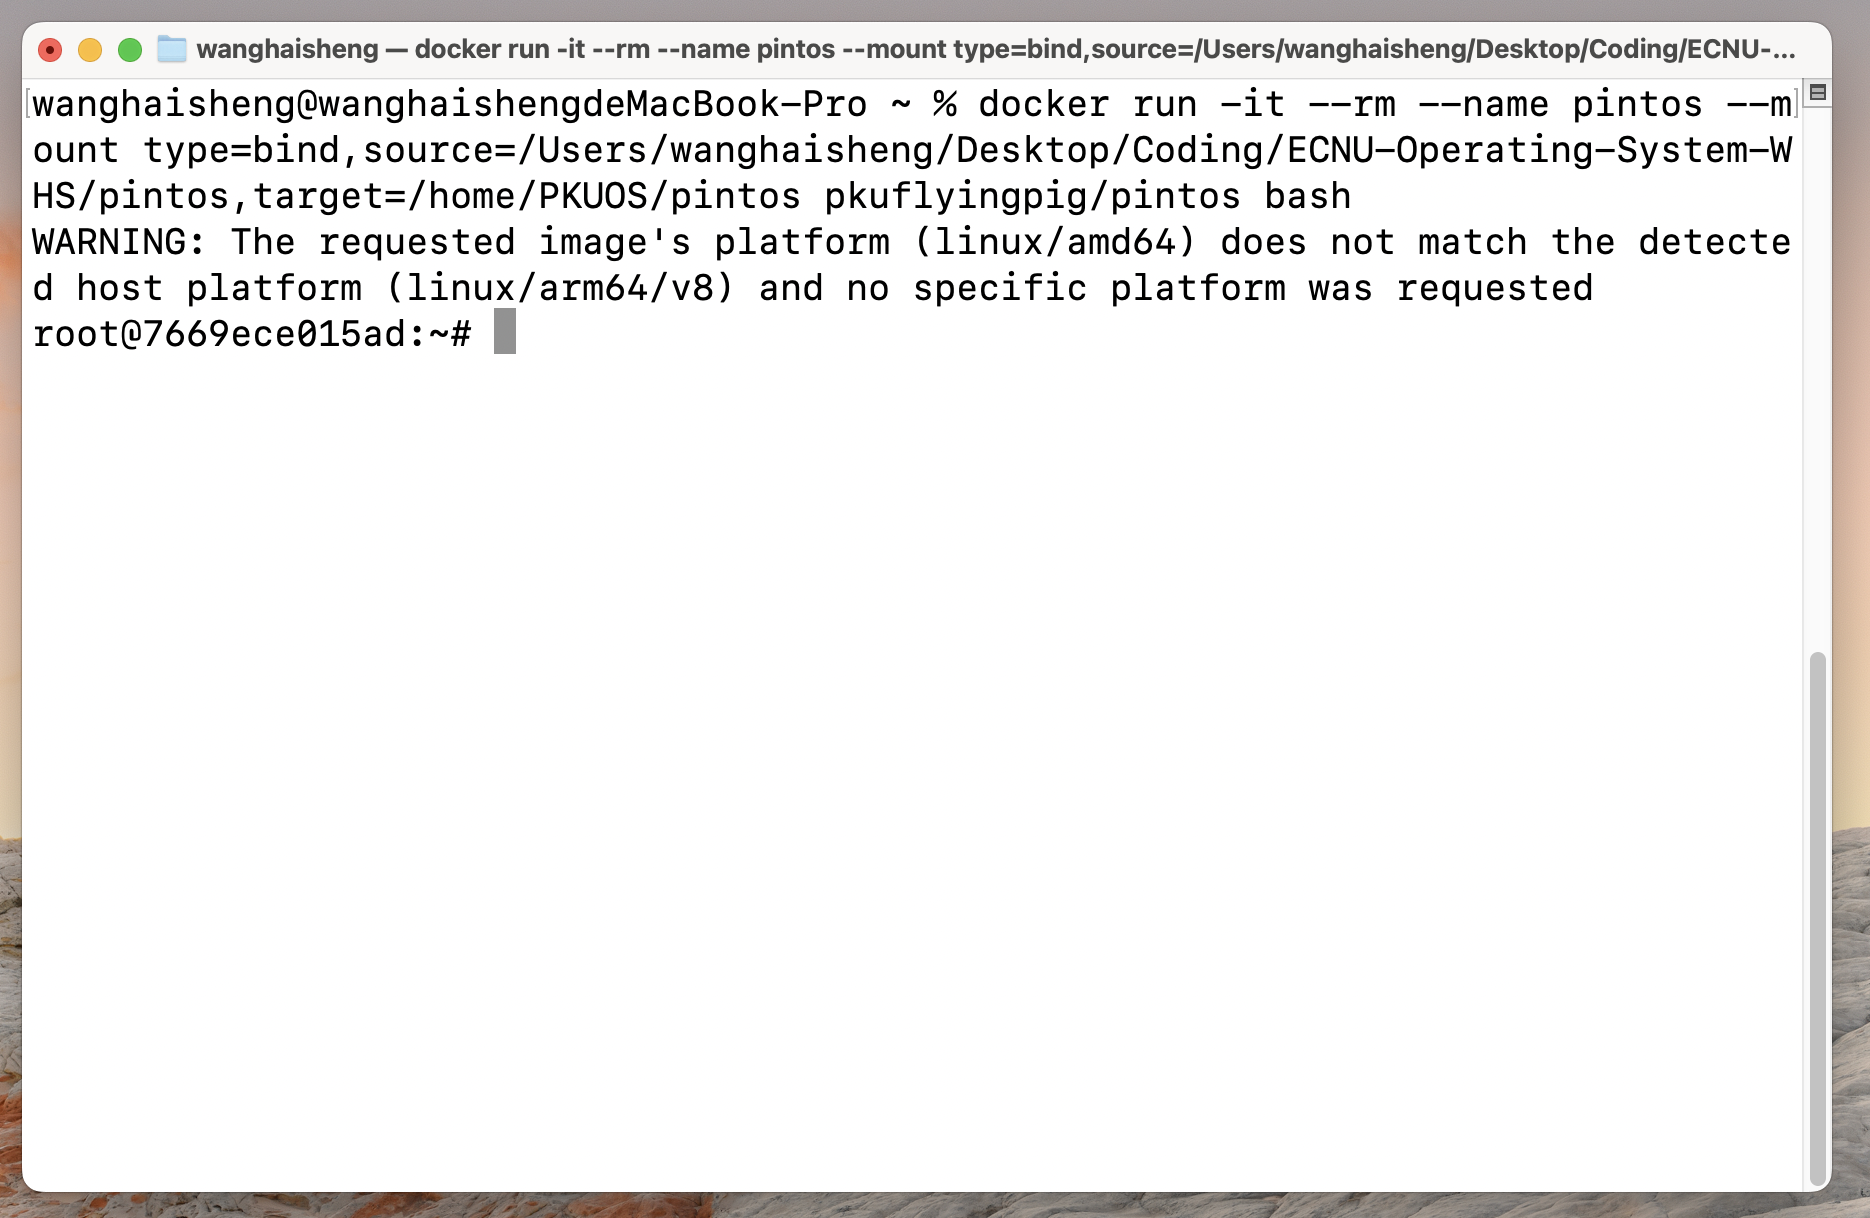
\includegraphics[width=0.9\textwidth]{img/run_docker.png}
	\caption{完成环境配置}
\end{figure}

\normalsize

\section{实验过程}

\subsection{PintOS源码解析}

Pintos 是一个专为教学设计的小型操作系统,其源代码结构清晰,功能简单,方便初学者学习。通过对 Pintos 源码目录的分析,我们可以了解到整个系统的组织方式。由于文件树状结构过于冗长,无法完整展示,所以这里采用层层深入的方法,管中窥豹。

\subsubsection{顶级目录}
在顶层目录下,可以找到以下几个重要文件:
\begin{itemize}
	\item \texttt{LICENSE}:包含了软件许可信息。
	\item \texttt{Makefile}:这是项目的主 Makefile 文件,定义了构建项目所需的所有规则。
	\item \texttt{Make.config}:配置文件,用于设置编译选项及路径等。
	\item \texttt{Makefile.build}、\texttt{Makefile.kernel}、\texttt{Makefile.userprog}:这些是针对内核和用户程序等不同组件的特定 Makefile 文件。
\end{itemize}

\subsubsection{源代码目录}
源代码被划分为几个子目录,每个都专注于操作系统的某个特定方面:
\begin{itemize}
	\item \texttt{devices/}:这里存放着设备驱动程序的实现,包括磁盘、键盘等硬件接口。
	\item \texttt{examples/}:提供了一些示例用户程序,帮助我们理解如何在 Pintos 上开发应用程序。
	\item \texttt{filesys/}:负责文件系统相关的功能,如磁盘格式化与文件读写。
	\item \texttt{lib/}:库函数集合,提供了许多通用的功能支持。
	\item \texttt{misc/}:一些辅助工具或脚本可能存放于此。
	\item \texttt{tests/}:测试用例集,用来确保 Pintos 各项功能的正确性。
	\item \texttt{threads/}:实现了多任务调度以及同步机制的核心线程系统。
	\item \texttt{userprog/}:处理用户进程相关的问题,比如加载和执行用户级程序。
	\item \texttt{utils/}:实用工具,通常与构建、调试或测试有关。
	\item \texttt{vm/}:虚拟内存管理模块,处理地址空间分配等问题。
\end{itemize}

\subsubsection{构建与测试}
当执行 \texttt{make} 命令时,顶层的 \texttt{Makefile} 会调用各个子目录下的 \texttt{Makefile} 来完成整个项目的编译,生成 Pintos 的可执行文件以及其他必要的二进制文件。对于测试来说,可以通过运行 \texttt{make check} 来自动执行所有预设的测试案例,并通过相应的检查脚本来验证结果是否符合预期。

\subsubsection{threads目录详解}
\texttt{threads/} 目录是 Pintos 操作系统中负责线程管理和调度的核心部分。它包含多个文件和子目录,每个都有其特定的功能。

\paragraph{根目录}
\begin{itemize}
	\item \texttt{Makefile 和 Make.vars} 用于定义编译规则和变量设置。
	\item \texttt{init.c 和 init.h} 初始化代码及相关的头文件,包含启动时线程系统的初始化逻辑。
	\item \texttt{interrupt.c 和 interrupt.h} 中断处理程序的实现。
	\item \texttt{intr-stubs.S 和 intr-stubs.h} 提供低级中断处理的支持。
	\item \texttt{io.h} 输入输出操作的头文件。
	\item \texttt{kernel.lds.S}] 定义了内核镜像的布局。
	\item \texttt{loader.S 和 loader.h} 引导加载器的汇编代码及其头文件。
	\item \texttt{malloc.c 和 malloc.h} 动态内存分配的实现。
	\item \texttt{palloc.c 和 palloc.h} 物理页帧分配器。
	\item \texttt{pte.h} 页表项相关的定义。
	\item \texttt{start.S} 内核的入口点。
	\item \texttt{switch.S 和 switch.h} 上下文切换代码。
	\item \texttt{synch.c 和 synch.h} 同步机制的实现,如锁、信号量等。
	\item \texttt{thread.c 和 thread.h} 线程管理的核心实现。
	\item \texttt{vaddr.h} 虚拟地址空间相关的定义。
\end{itemize}

\paragraph{子目录}

\begin{itemize}
	\item \texttt{build} 目录是编译过程中生成的中间文件和最终二进制文件存放的地方,包括目标文件 .o 文件、调试符号文件 .d 文件、链接后的内核镜像 \texttt{kernel.bin} 等。
\end{itemize}

\subsubsection{/src/tests/threads目录详解}
\texttt{/src/tests/threads} 目录包含了 Pintos 操作系统中与线程相关的测试用例。

\paragraph{测试用例文件(.c 文件)}
这些 C 语言编写的测试程序代表独立的测试用例,通过调用 Pintos API 来创建线程、设置定时器、修改优先级等,并执行一系列操作来测试特定的功能。

\paragraph{测试结果检查脚本(.ck 文件)}
这些 Perl 脚本用来自动检查测试用例的输出是否符合预期。当运行 \texttt{make check} 或者手动运行单个测试时,Pintos 会将测试输出保存到文件中,然后使用相应的 .ck 脚本来验证这些输出。

\paragraph{其他文件}
\begin{itemize}
	\item \texttt{Make.tests} 定义了如何编译和链接测试用例。
	\item \texttt{tests.c 和 tests.h} 主要的测试驱动代码。
	\item \texttt{Rubric.alarm, Rubric.mlfqs, Rubric.priority} 记录评分标准或测试指南的文本文件。
	\item \texttt{Grading} 可能是一个目录,包含了关于测试评分的信息。
	\item \texttt{alarm.pm, mlfqs.pm} Perl 模块文件,提供了一些辅助函数或数据结构。
\end{itemize}

\subsubsection{/src/tests目录详解}
\texttt{/src/tests} 目录是 Pintos 操作系统中用于存放各种测试用例和相关脚本的地方。

\paragraph{文件}
\begin{itemize}
	\item \texttt{Make.tests} 定义了如何编译和运行所有测试用例。
	\item \texttt{arc4.c, arc4.h} 实现了 ARC4 加密算法。
	\item \texttt{cksum.c, cksum.h, cksum.pm} 提供计算校验和的功能。
	\item \texttt{lib.c, lib.h} 自定义的库函数。
	\item \texttt{lib.pm} Perl 模块,包含通用的辅助函数。
	\item \texttt{main.c, main.h} 主测试程序的框架。
	\item \texttt{make-grade} 用于自动评分的脚本。
	\item \texttt{random.pm} 提供随机数生成的功能。
	\item \texttt{tests.pm} 包含运行测试所需的公共函数或数据结构。
\end{itemize}

\paragraph{子目录}
\begin{itemize}
	\item \texttt{Algorithm} 与特定算法相关的测试。
	\item \texttt{filesys} 文件系统相关的测试用例。
	\item \texttt{threads} 线程管理相关的测试用例。
	\item \texttt{userprog} 用户进程相关的测试用例。
	\item \texttt{vm} 虚拟内存管理相关的测试用例。
\end{itemize}

\subsection{实现\texttt{hello-world}函数}

我将通过以下四个步骤来实现一个名为\texttt{hello-world}的测试函数:创建新的测试文件、更新测试配置文件、修改Makefile、验证结果。

\subsubsection{新建\texttt{hello-world.c}文件}
首先,我在\texttt{src/test/threads/}目录下创建了一个新文件\texttt{helloworld.c}。在这个文件里,我定义了一个简单的测试函数,它仅打印出\texttt{hello world!}。下面是该文件的内容:

\begin{figure}[H]
	\centering
	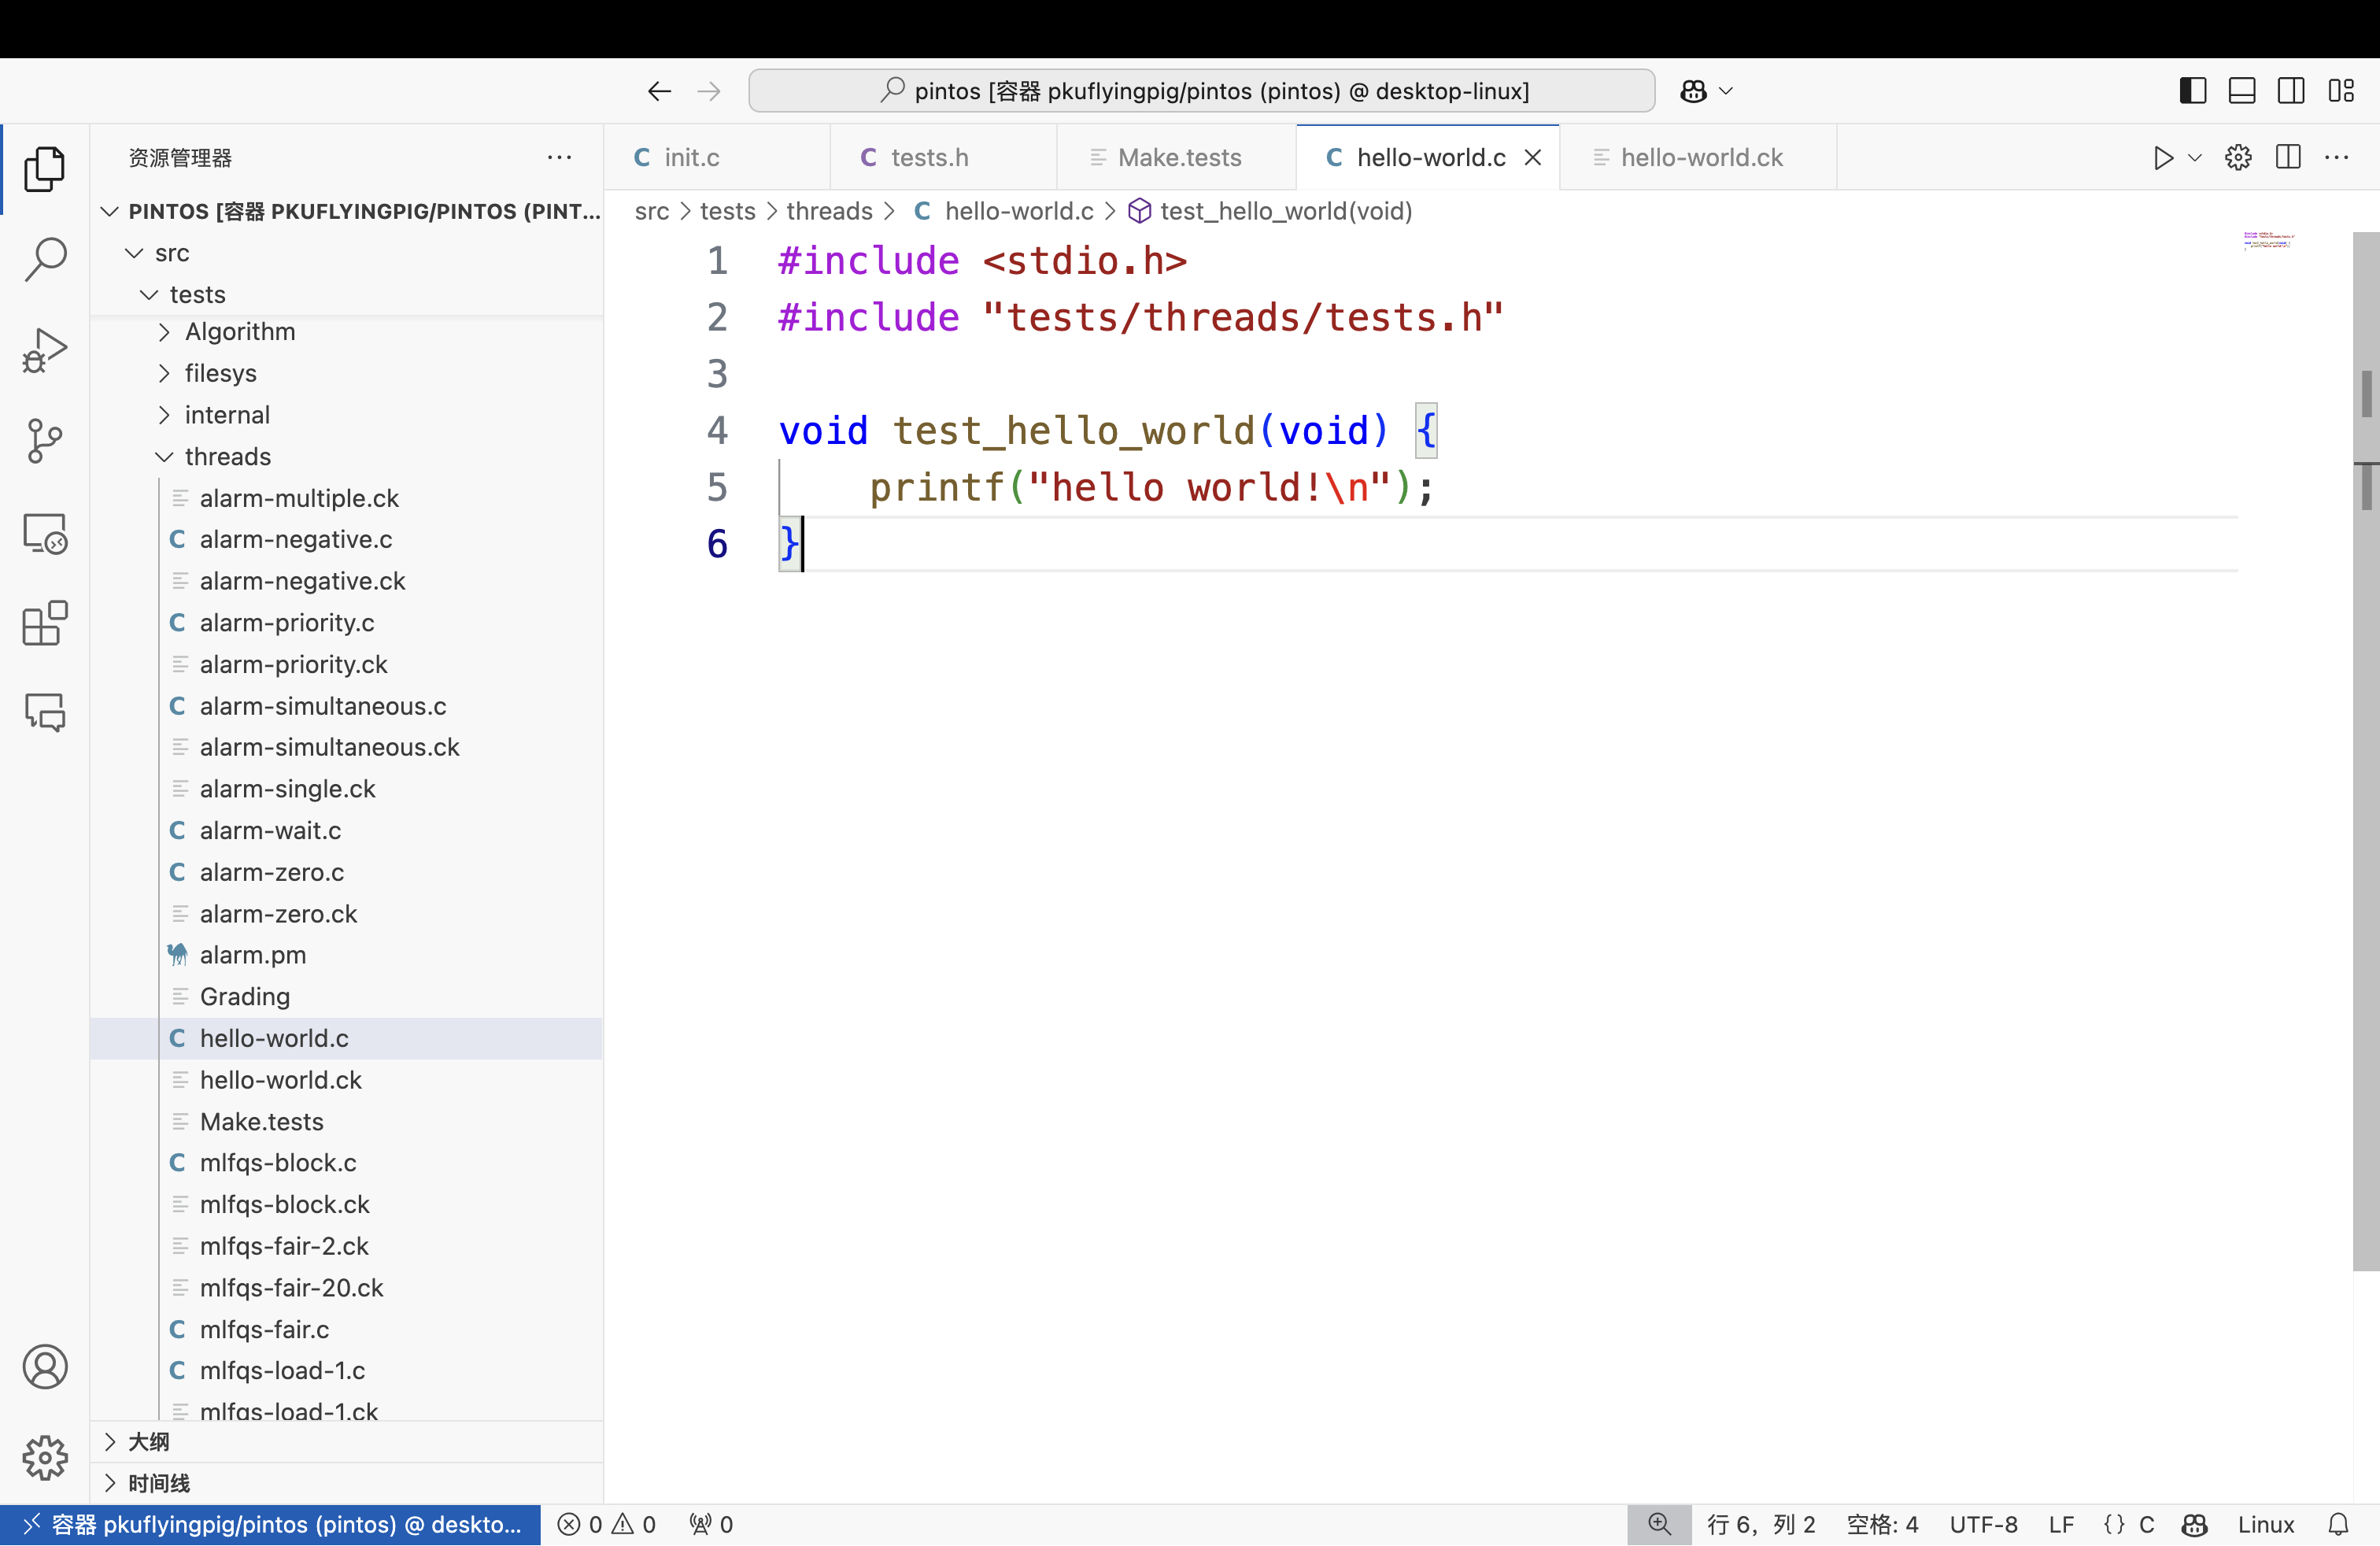
\includegraphics[width=0.8\textwidth]{img/helloworld.png}
	\caption{新建\texttt{hello-world.c}文件}
\end{figure}

\subsubsection{修改配置文件}
为了让Pintos知道这个新的测试函数,我更新了\texttt{src/test/threads/test.c}和\texttt{src/test/threads/test.h}以引入我的新函数。在\texttt{test.h}中我添加了外部声明,在\texttt{test.c}中的\texttt{struct test tests[]}数组里也添加了我的新测试项。我所做的修改如下图所示。

\begin{figure}[H]
	\centering
	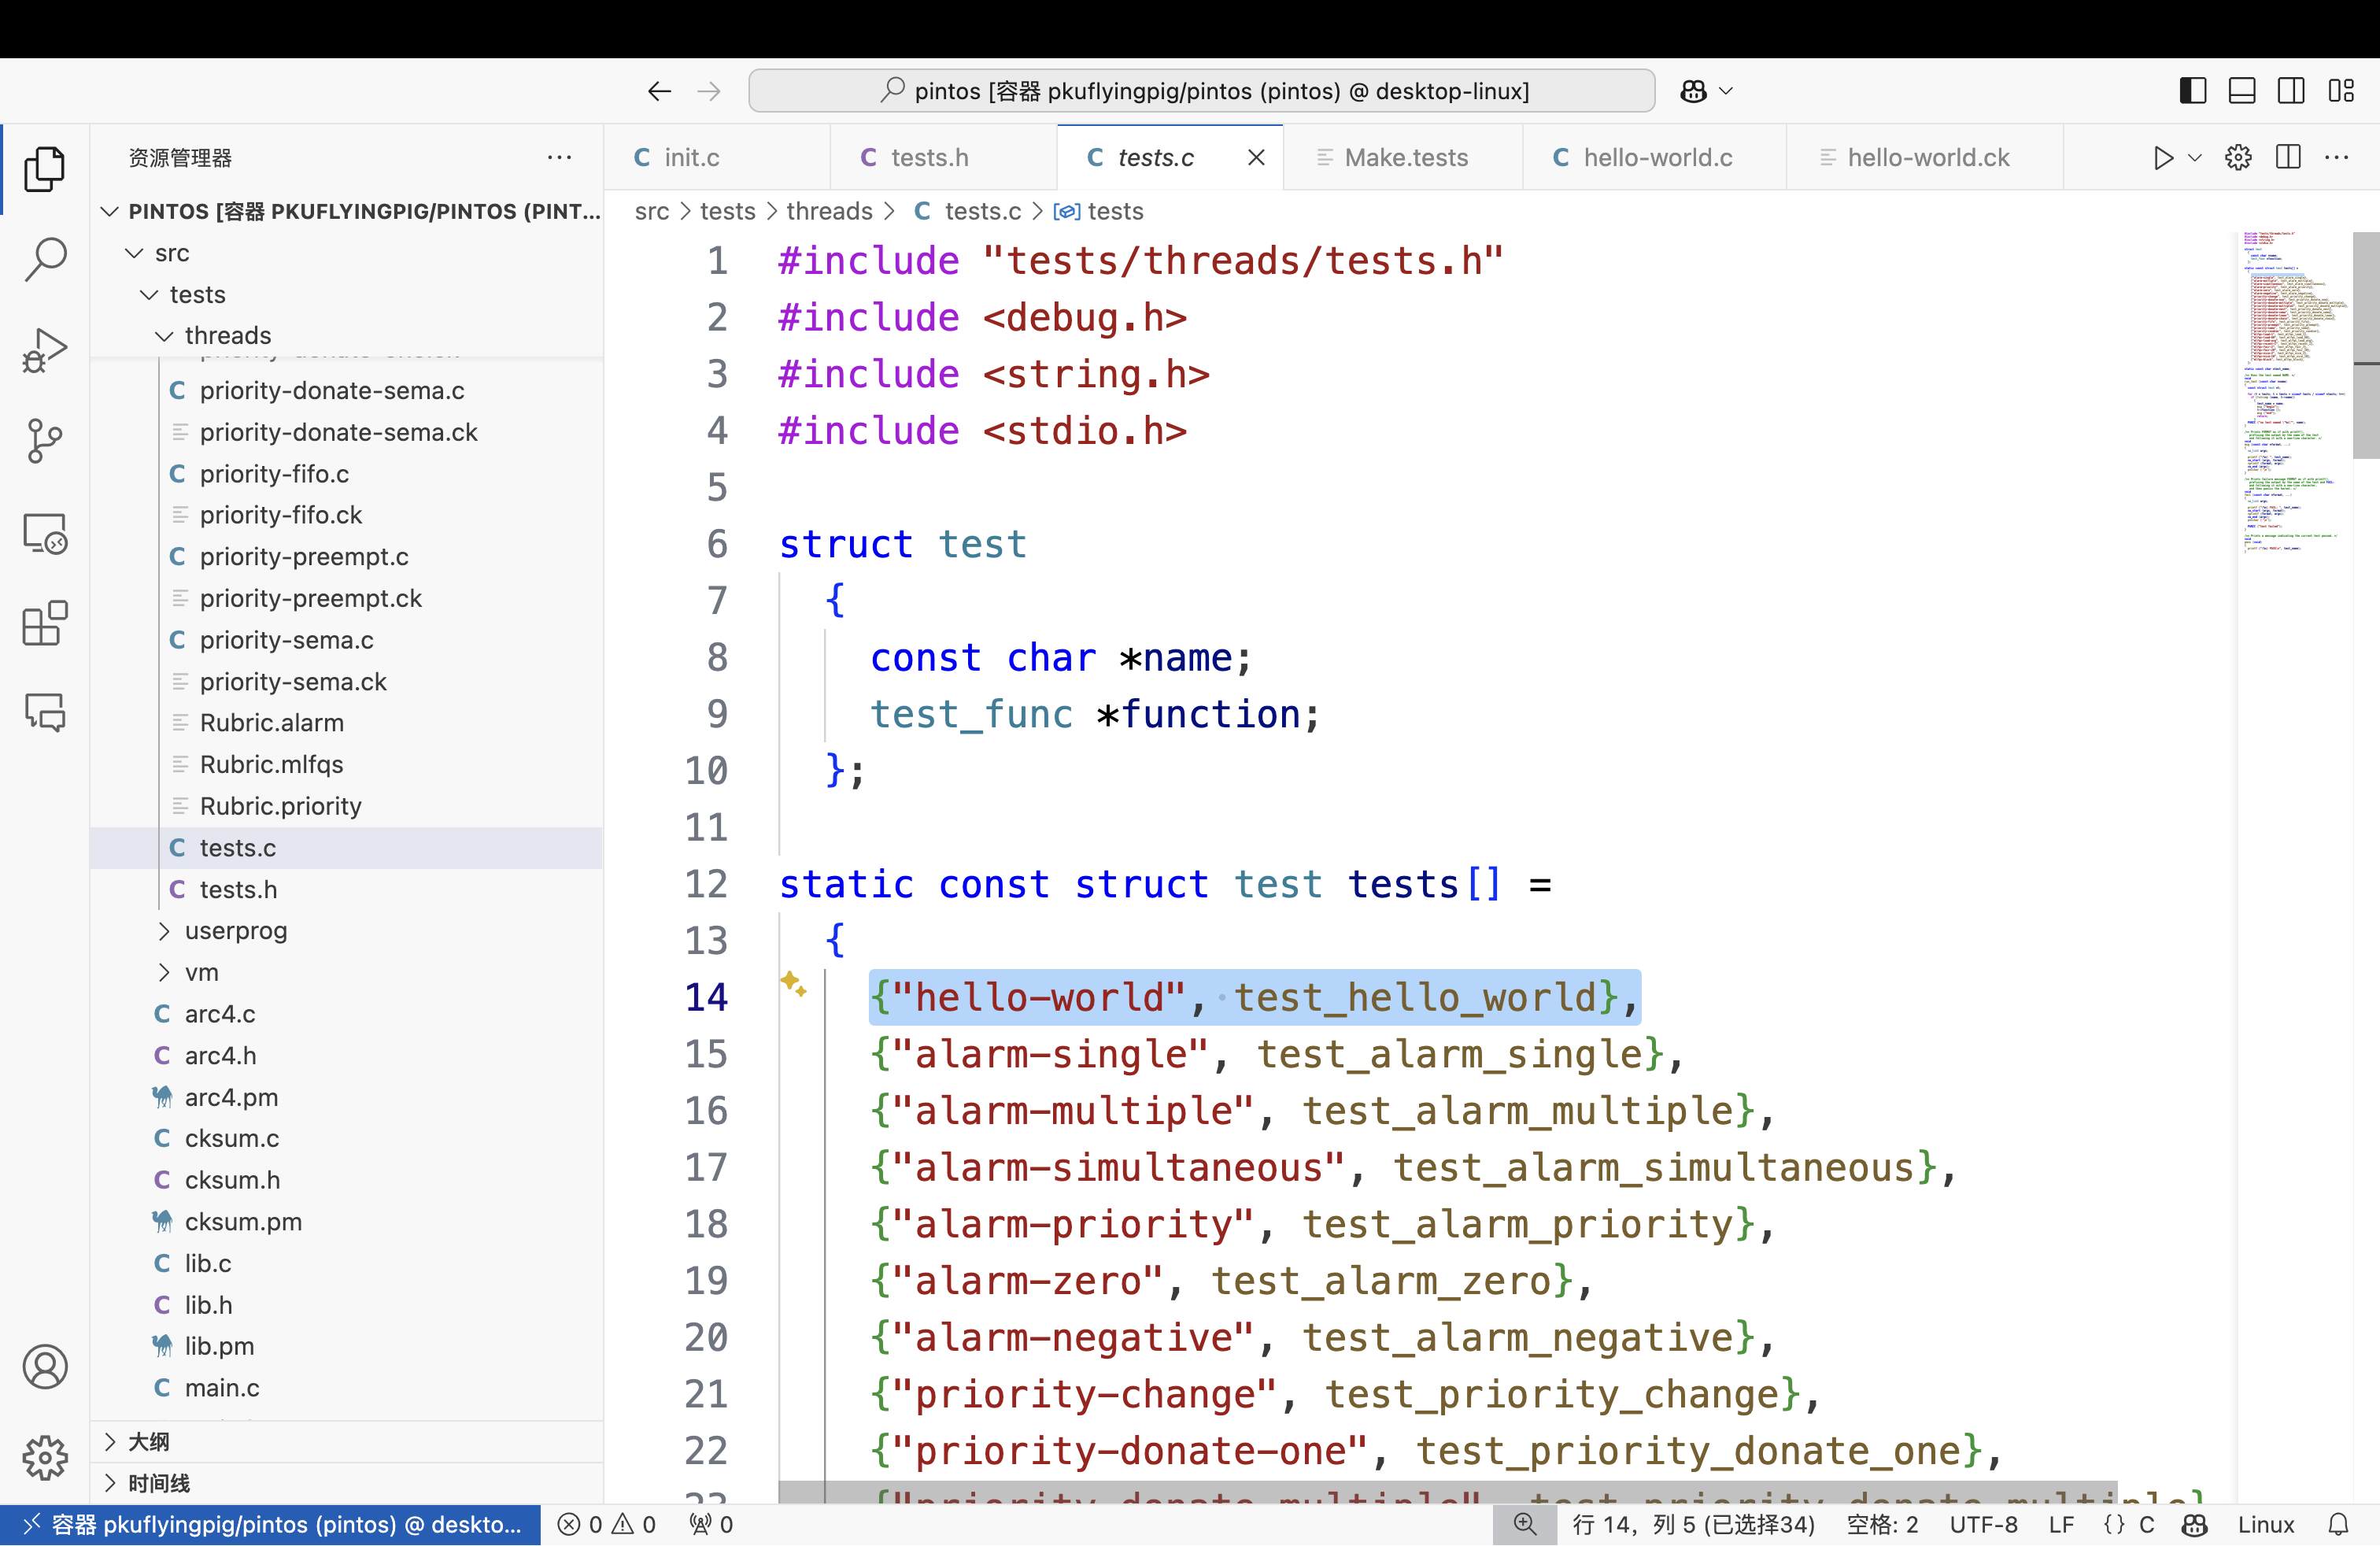
\includegraphics[width=0.8\textwidth]{img/testsc.png}
	\caption{修改\texttt{tests.c}文件}
\end{figure}

\begin{figure}[H]
	\centering
	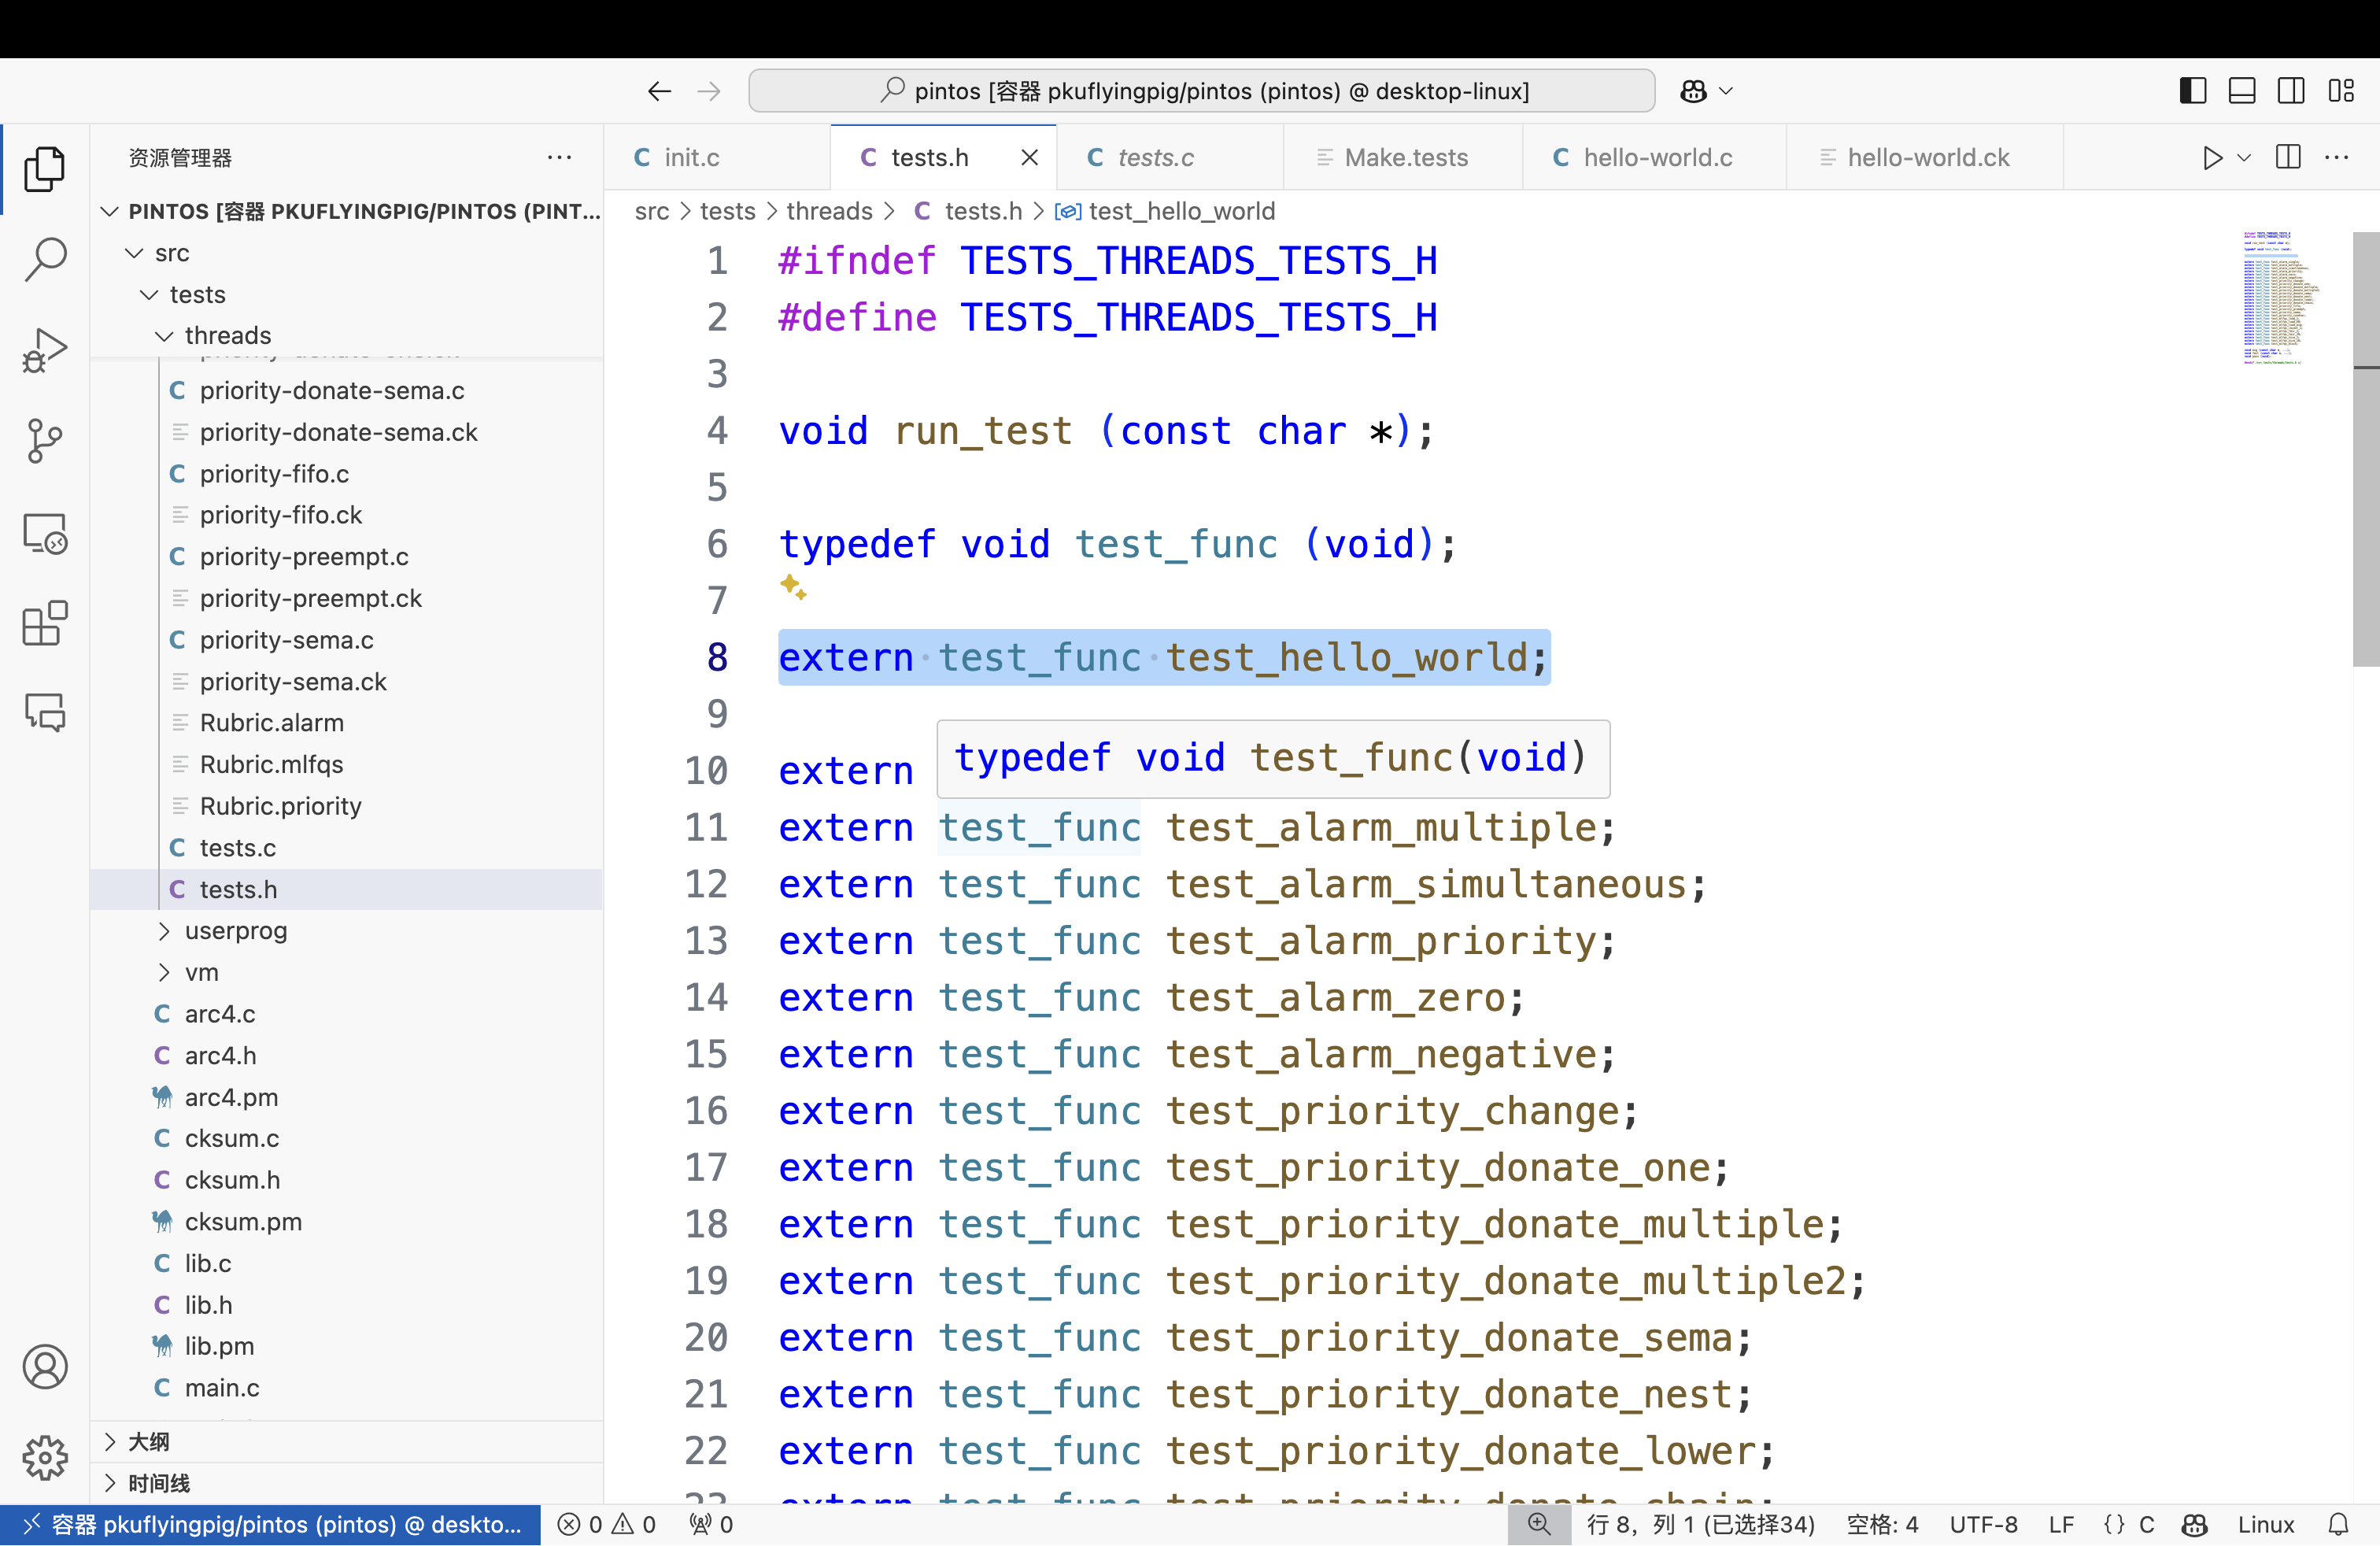
\includegraphics[width=0.8\textwidth]{img/testsh.png}
	\caption{修改\texttt{tests.h}文件}
\end{figure}

\subsubsection{修改Makefile}
为了编译新添加的测试文件,我还需要修改\texttt{src/test/threads/Make.tests}文件,在其中添加对\texttt{helloworld.c}的引用,并在我的测试名称列表中加入\texttt{hello-world},如下图所示。

\begin{figure}[H]
	\centering
	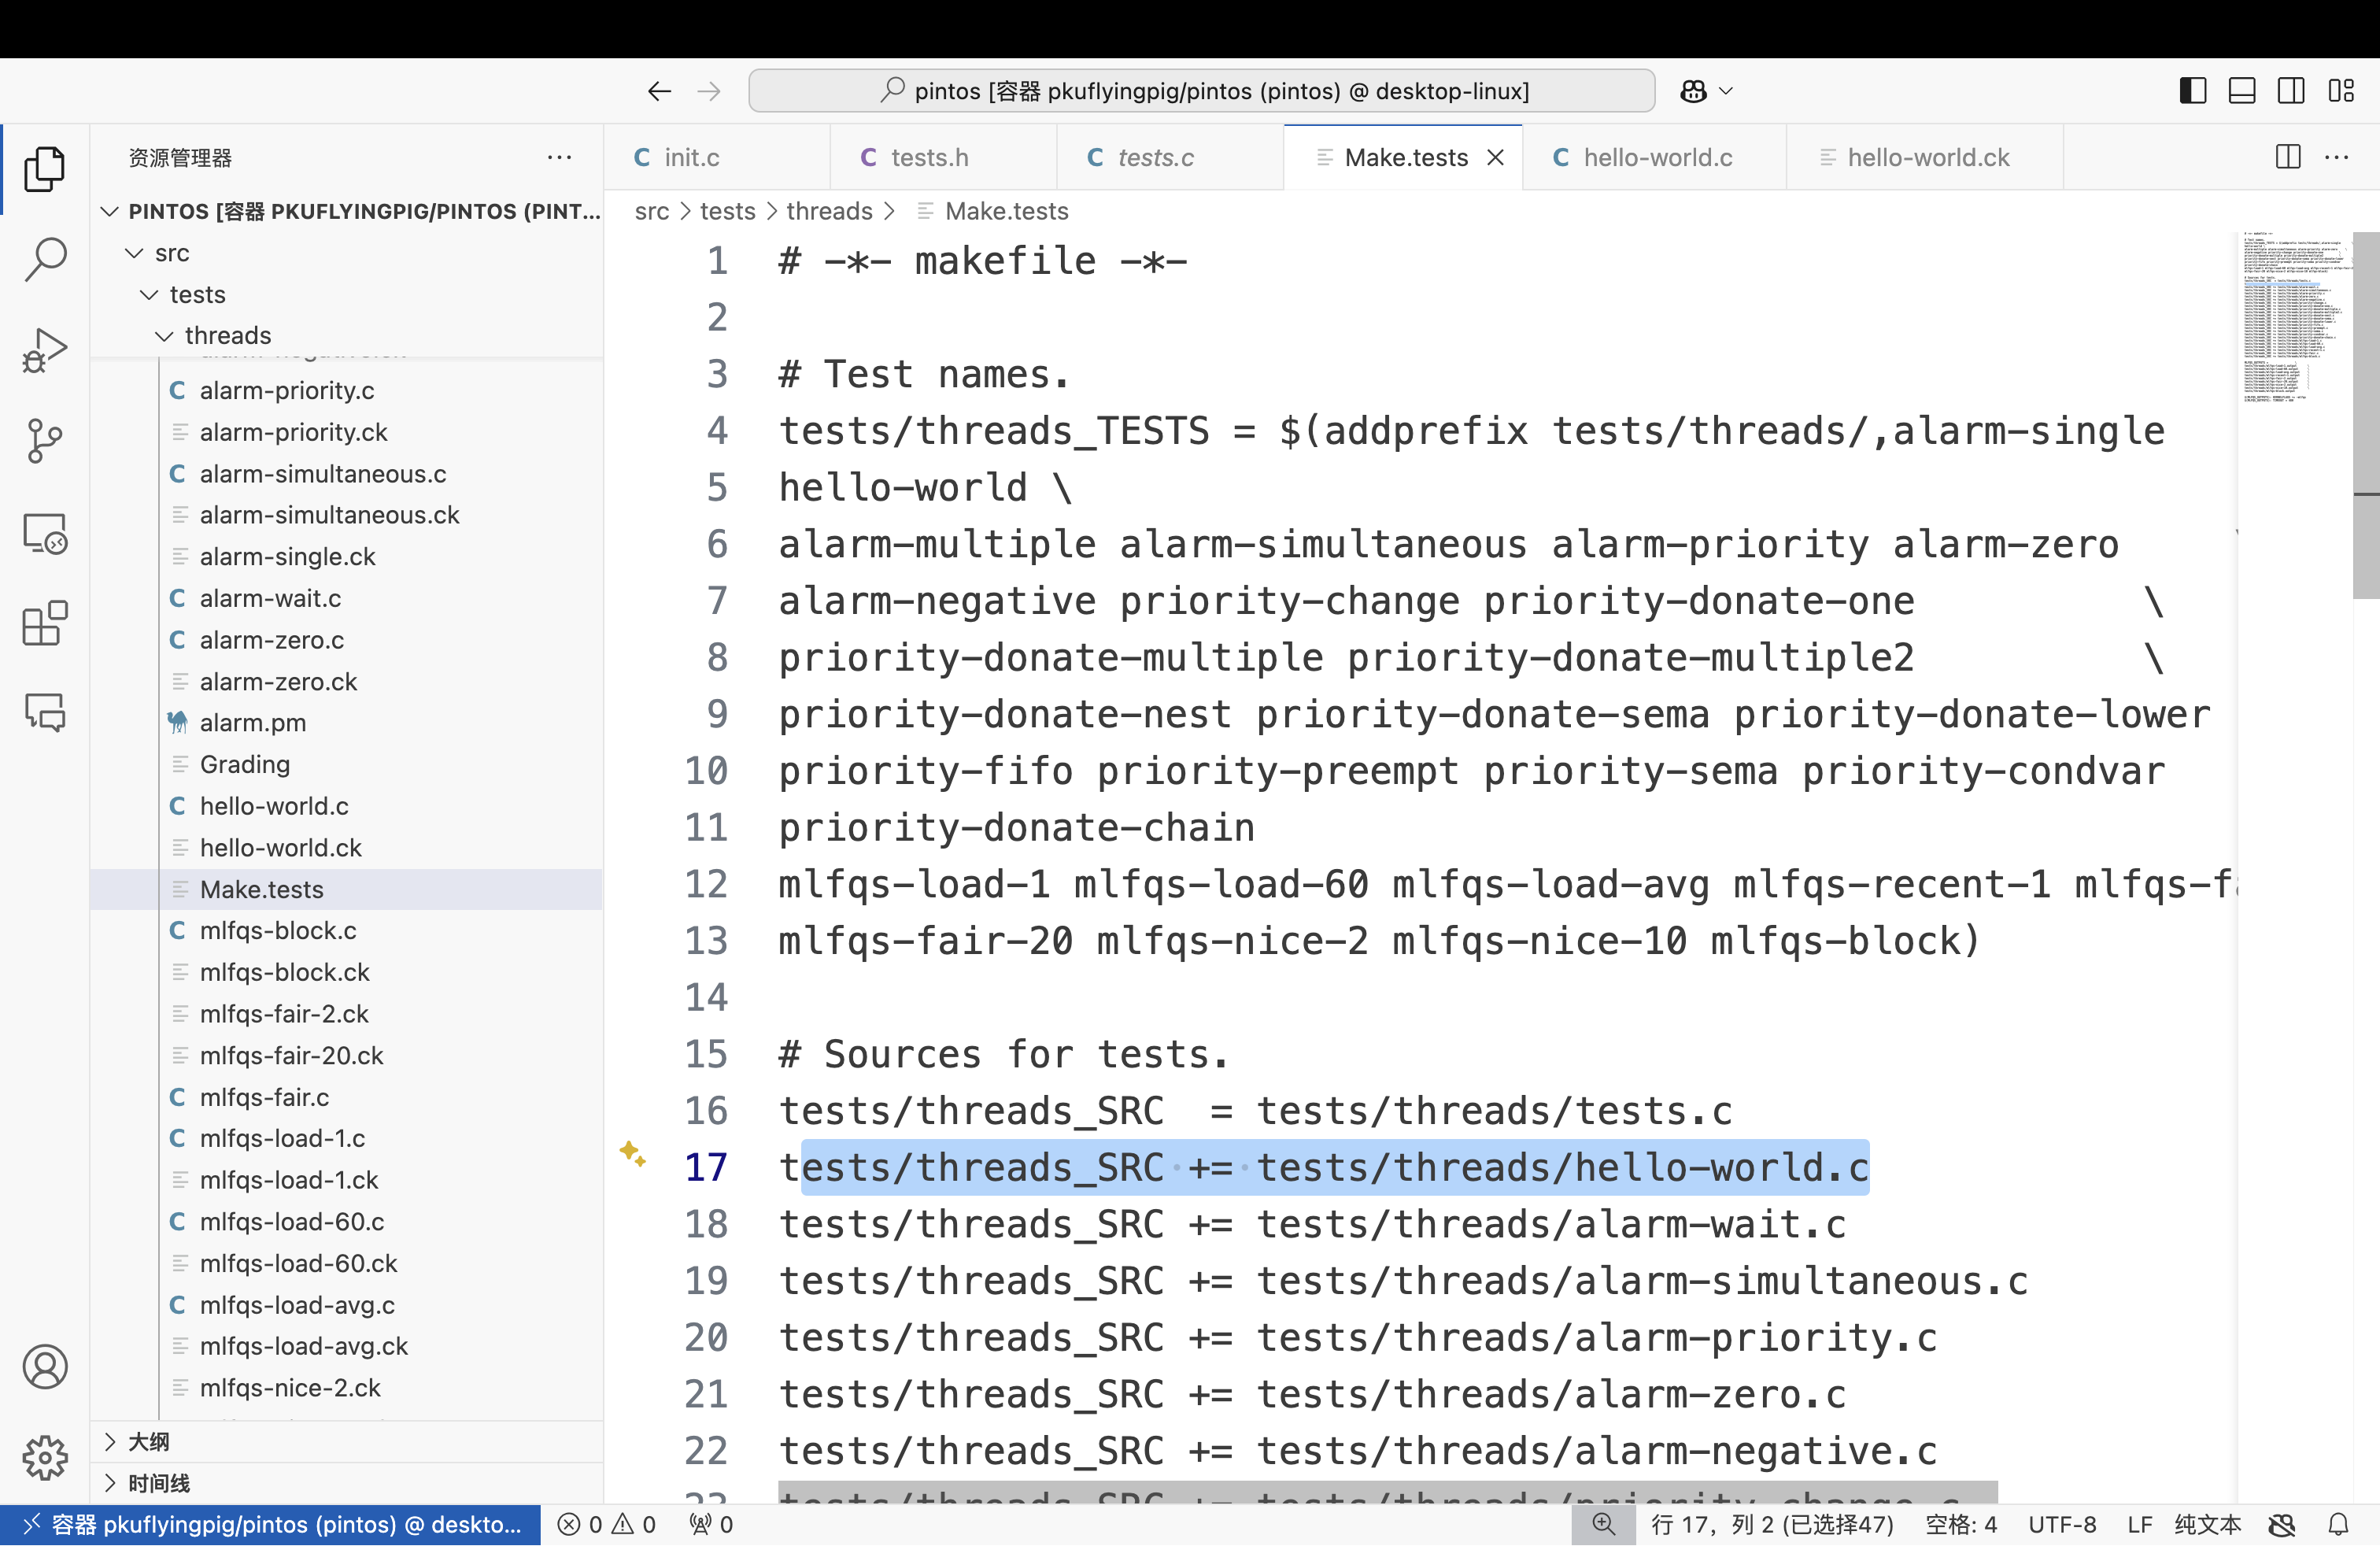
\includegraphics[width=0.8\textwidth]{img/maketests.png}
	\caption{修改\texttt{Make.tests}文件}
\end{figure}

\subsubsection{验证结果}

在命令行中输入\texttt{pintos -- -q run hello-world}命令,运行结果如下图所示。

\begin{figure}[H]
	\centering
	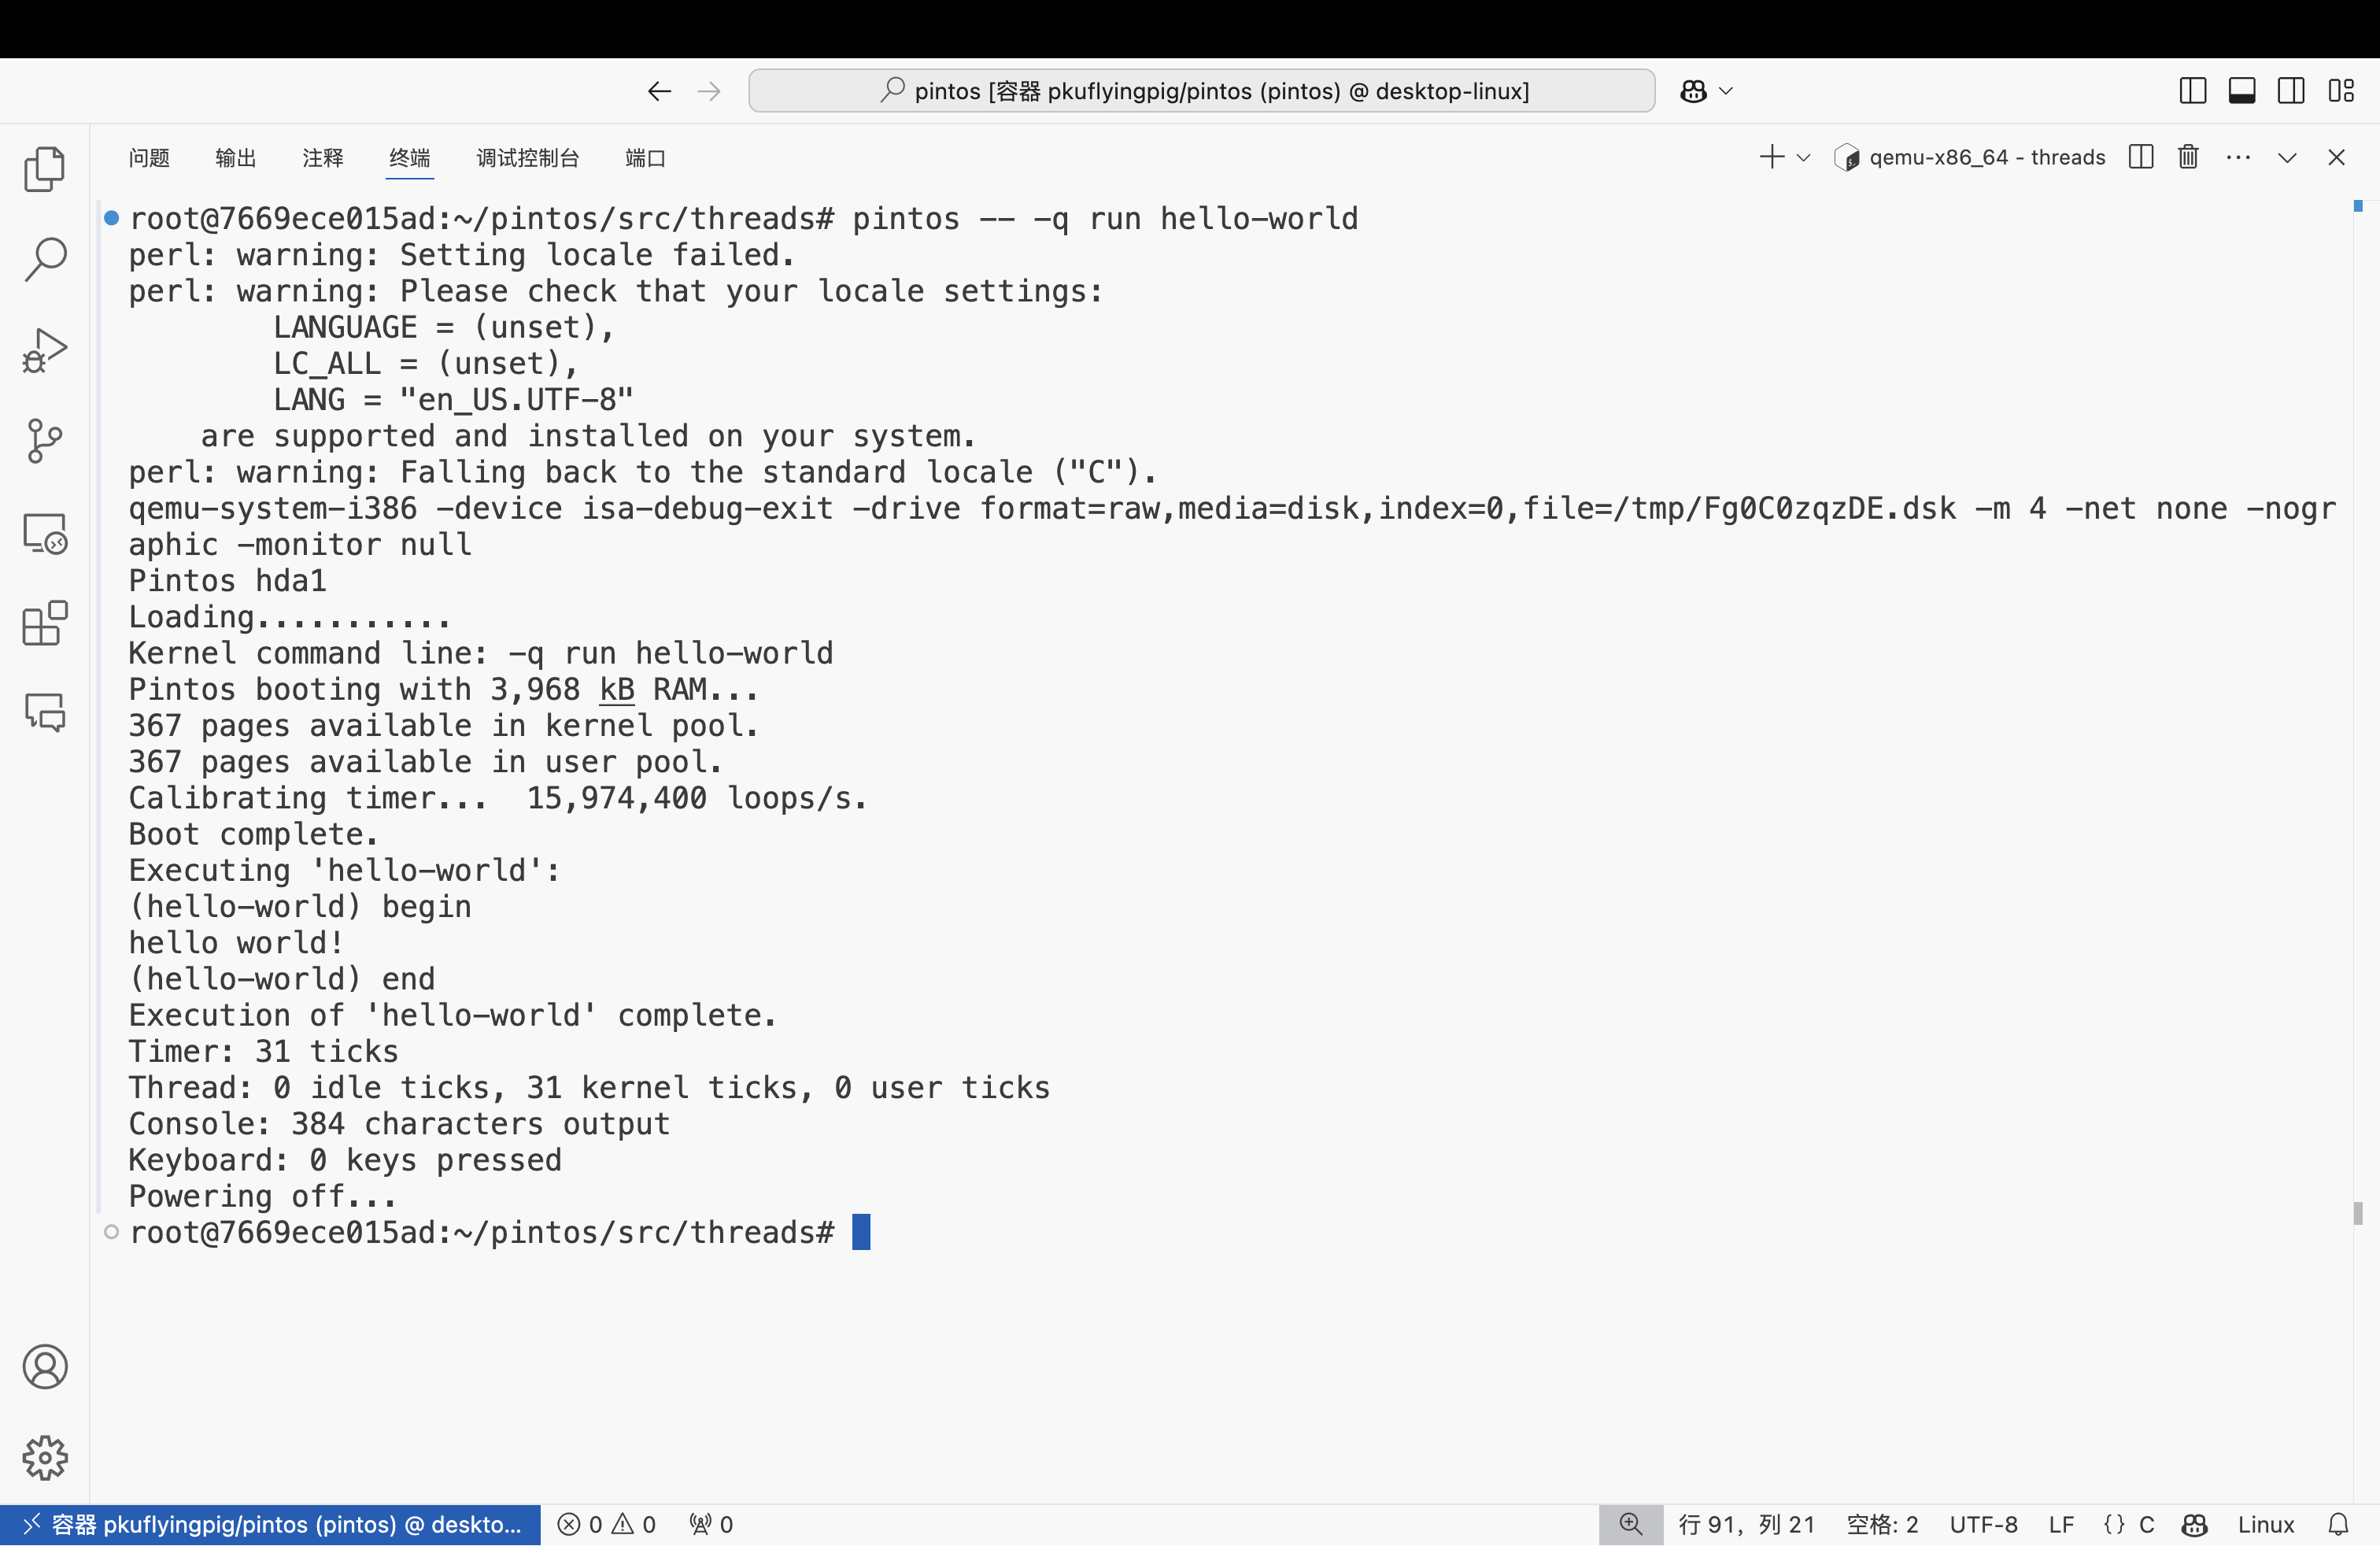
\includegraphics[width=0.8\textwidth]{img/run_helloworld.png}
	\caption{运行\texttt{hello-world}}
\end{figure}

至此,\texttt{hello-world}函数成功添加。

\subsection{修改测试程序}

为了让PintOS测试系统识别\texttt{hello-world}函数并跑分,需要新建\texttt{hello-world.ck}文件,并添加\texttt{hello-world}的预期结果。如下图所示:

\begin{figure}[H]
	\centering
	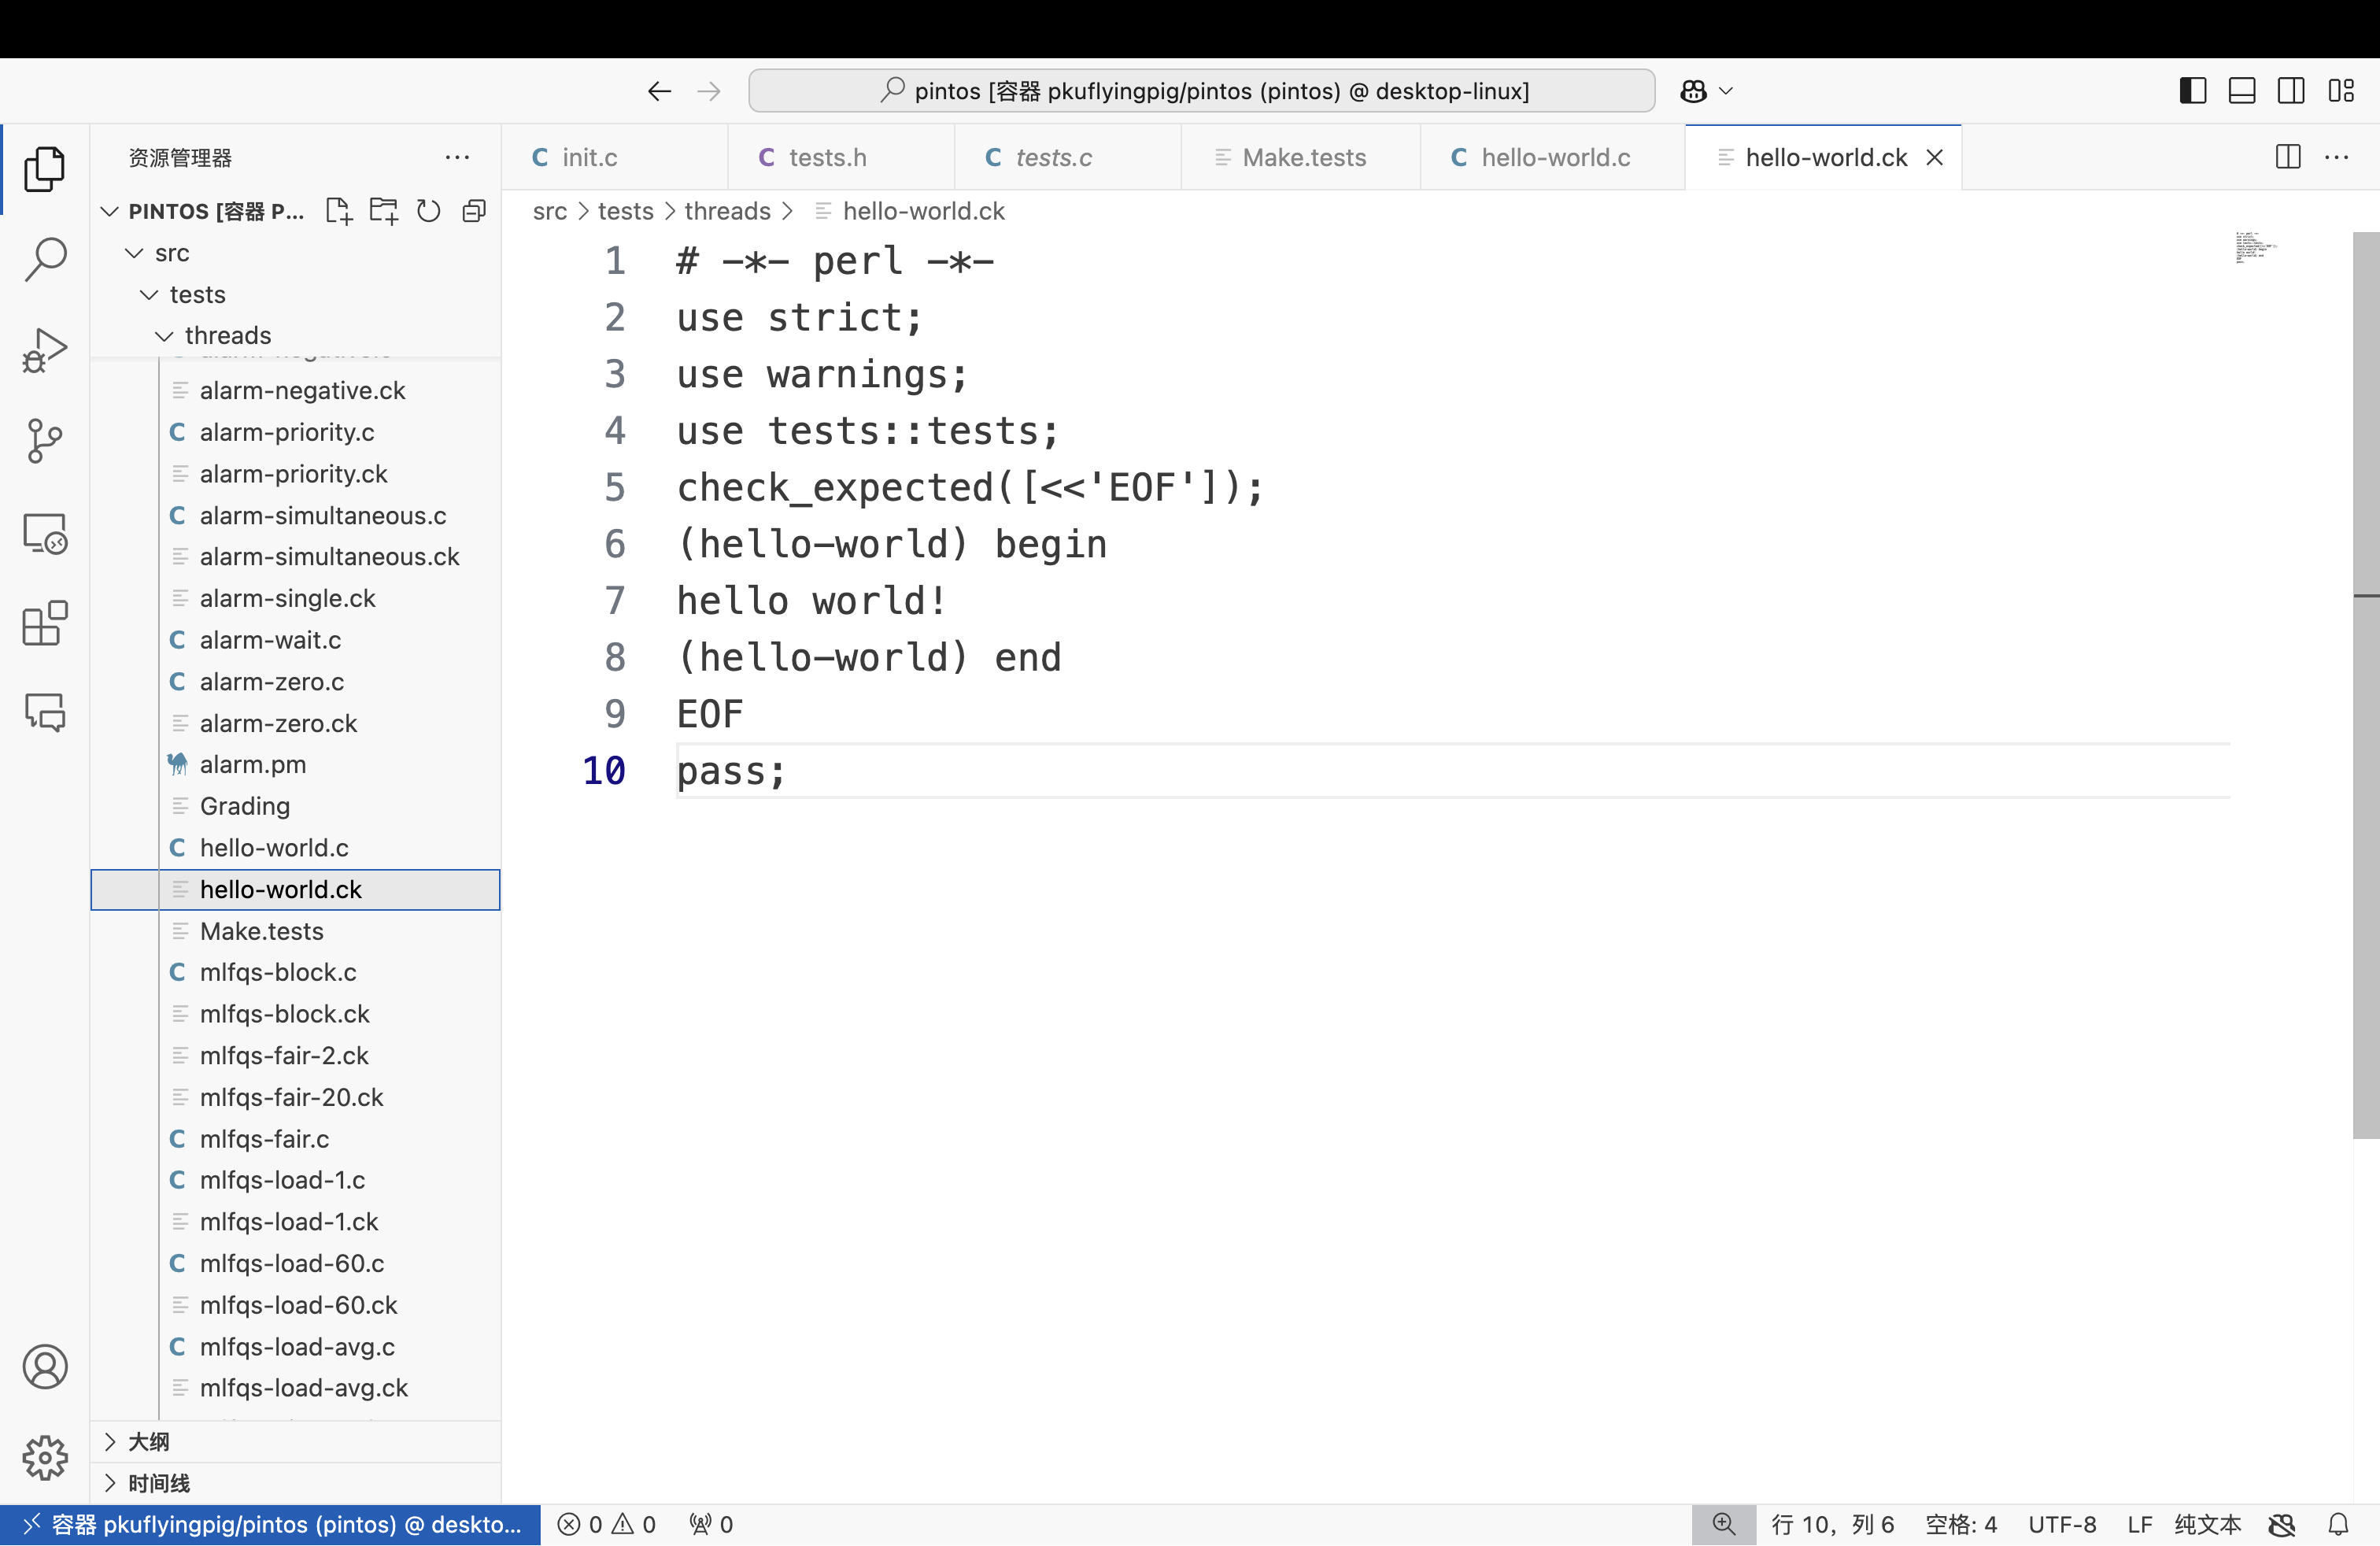
\includegraphics[width=0.8\textwidth]{img/helloworldck.png}
	\caption{新建\texttt{hello-world.ck}}
\end{figure}

修改完成后,执行\texttt{make check}命令,发现通过了测试,如下图:

\begin{figure}[H]
	\centering
	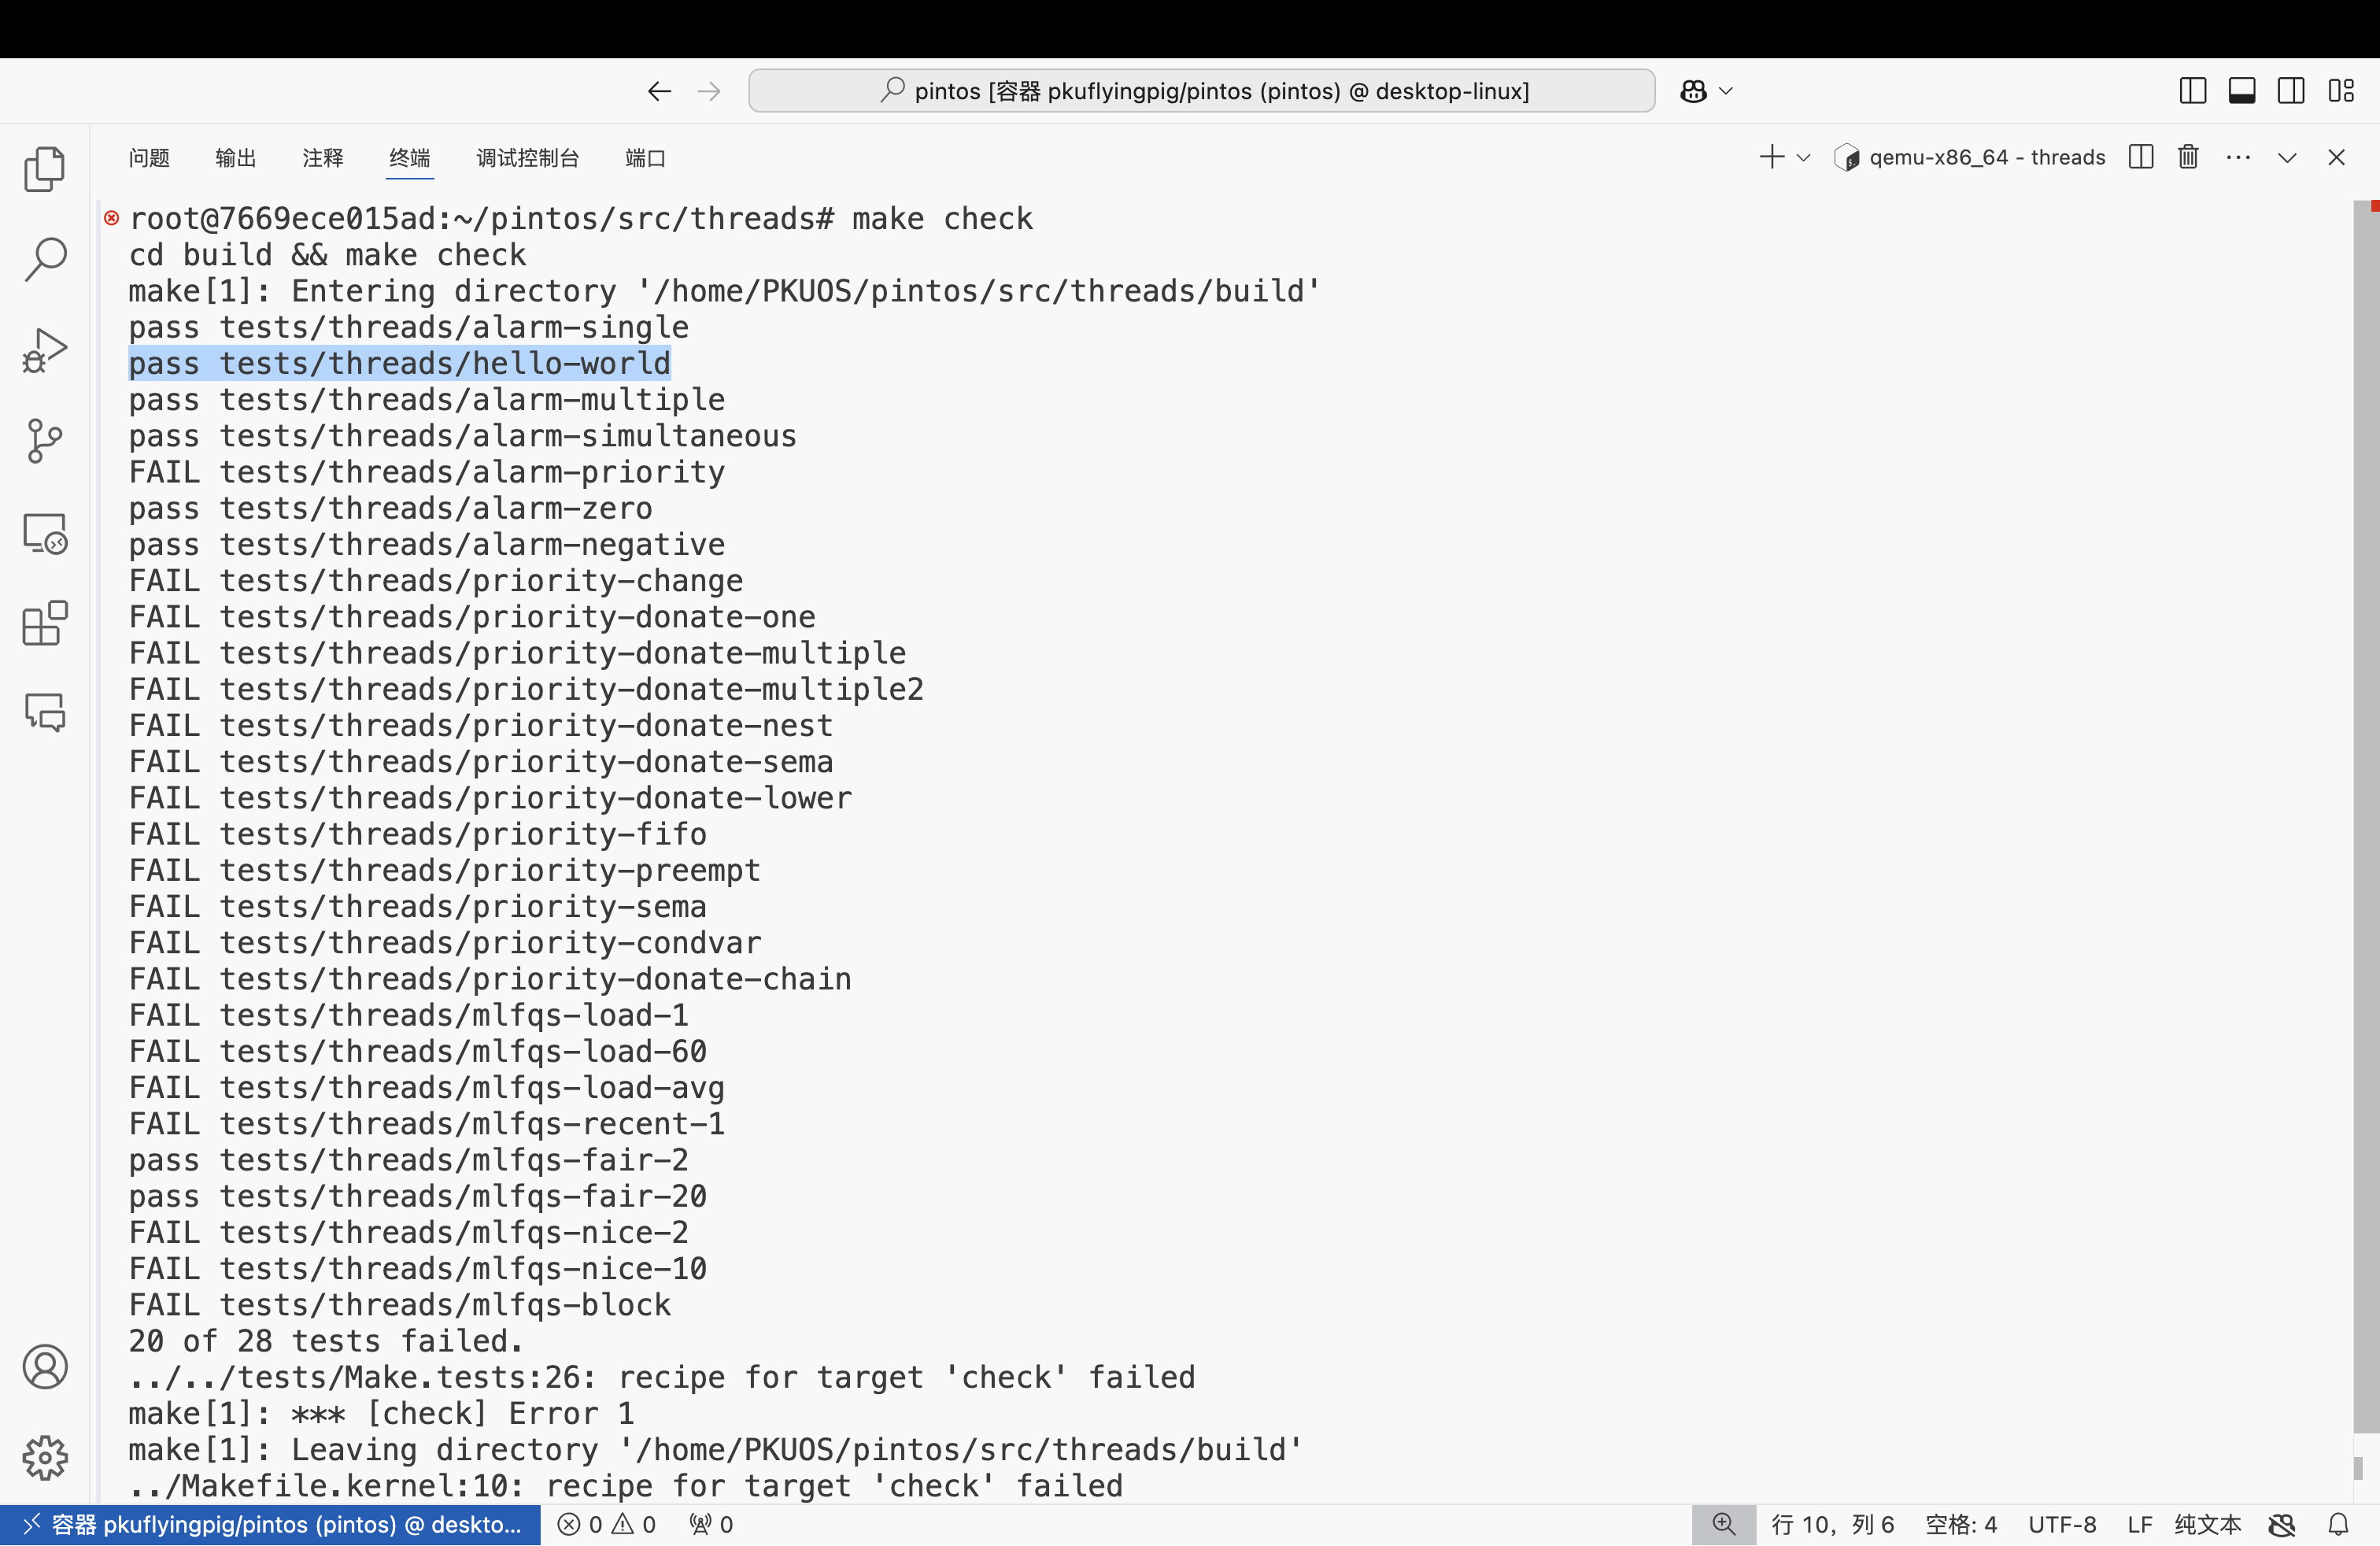
\includegraphics[width=0.8\textwidth]{img/makecheck.png}
	\caption{\texttt{make check}测试}
\end{figure}

到这里,本次实验全部完成。

\normalsize

\section{实验总结}

谈一谈我的收获吧。

第一个是\texttt{Visual Studio Code}和\texttt{Git}的使用,虽然受限于篇幅没有写在这份实验报告中,但这个学习过程以及学习所得都让我离优秀的程序员更近了一步。以前我用的是\texttt{IDE},现在才发现一个插件丰富的文本编辑器竟能这么好用;至于\texttt{Git},很久以前就在电脑上安装了,但一直没用过,知道这次实验才真正在\texttt{GitHub}创建项目。不出意外的话,以后我的工作流就会使用\texttt{Visual Studio Code}和\texttt{Git}啦。

第二个是“知其然必先知其所以然”的道理。在我最初的尝试中,我在\texttt{hello-world.c}文件中使用了\texttt{int main(void) {}}这样的常规结构,然后一直无法编译运行。根据错误信息,我搜集了大量PintOS源码结构相关的资料(既本报告的“PintOS源码解析”部分),才把上面的错误成正确的:\texttt{void hello-world(void) {}}。直到这时,我才开始理解多文件联合编译、系统级Make的奥秘。

\normalsize

\section{附录:修改后的代码}

\begin{lstlisting}[language=C, title=\texttt{hello-world.c}]
	#include <stdio.h>
	#include "tests/threads/tests.h"
	
	void test_hello_world(void) {
		printf("hello world!\n");
	}
\end{lstlisting}

\begin{lstlisting}[language=C, title=\texttt{test.c}]
	#include "tests/threads/tests.h"
	#include <debug.h>
	#include <string.h>
	#include <stdio.h>
	
	struct test 
	{
		const char *name;
		test_func *function;
	};
	
	static const struct test tests[] = 
	{
		{"hello-world", test_hello_world},
		{"alarm-single", test_alarm_single},
		{"alarm-multiple", test_alarm_multiple},
		{"alarm-simultaneous", test_alarm_simultaneous},
		{"alarm-priority", test_alarm_priority},
		{"alarm-zero", test_alarm_zero},
		{"alarm-negative", test_alarm_negative},
		{"priority-change", test_priority_change},
		{"priority-donate-one", test_priority_donate_one},
		{"priority-donate-multiple", test_priority_donate_multiple},
		{"priority-donate-multiple2", test_priority_donate_multiple2},
		{"priority-donate-nest", test_priority_donate_nest},
		{"priority-donate-sema", test_priority_donate_sema},
		{"priority-donate-lower", test_priority_donate_lower},
		{"priority-donate-chain", test_priority_donate_chain},
		{"priority-fifo", test_priority_fifo},
		{"priority-preempt", test_priority_preempt},
		{"priority-sema", test_priority_sema},
		{"priority-condvar", test_priority_condvar},
		{"mlfqs-load-1", test_mlfqs_load_1},
		{"mlfqs-load-60", test_mlfqs_load_60},
		{"mlfqs-load-avg", test_mlfqs_load_avg},
		{"mlfqs-recent-1", test_mlfqs_recent_1},
		{"mlfqs-fair-2", test_mlfqs_fair_2},
		{"mlfqs-fair-20", test_mlfqs_fair_20},
		{"mlfqs-nice-2", test_mlfqs_nice_2},
		{"mlfqs-nice-10", test_mlfqs_nice_10},
		{"mlfqs-block", test_mlfqs_block},
	};
	
	static const char *test_name;
	
	/** Runs the test named NAME. */
	void
	run_test (const char *name) 
	{
		const struct test *t;
		
		for (t = tests; t < tests + sizeof tests / sizeof *tests; t++)
		if (!strcmp (name, t->name))
		{
			test_name = name;
			msg ("begin");
			t->function ();
			msg ("end");
			return;
		}
		PANIC ("no test named \"%s\"", name);
	}
	
	/** Prints FORMAT as if with printf(),
	prefixing the output by the name of the test
	and following it with a new-line character. */
	void
	msg (const char *format, ...) 
	{
		va_list args;
		
		printf ("(%s) ", test_name);
		va_start (args, format);
		vprintf (format, args);
		va_end (args);
		putchar ('\n');
	}
	
	/** Prints failure message FORMAT as if with printf(),
	prefixing the output by the name of the test and FAIL:
	and following it with a new-line character,
	and then panics the kernel. */
	void
	fail (const char *format, ...) 
	{
		va_list args;
		
		printf ("(%s) FAIL: ", test_name);
		va_start (args, format);
		vprintf (format, args);
		va_end (args);
		putchar ('\n');
		
		PANIC ("test failed");
	}
	
	/** Prints a message indicating the current test passed. */
	void
	pass (void) 
	{
		printf ("(%s) PASS\n", test_name);
	}
\end{lstlisting}

\begin{lstlisting}[language=C, title=\texttt{test.h}]
	#ifndef TESTS_THREADS_TESTS_H
	#define TESTS_THREADS_TESTS_H
	
	void run_test (const char *);
	
	typedef void test_func (void);
	
	extern test_func test_hello_world;
	
	extern test_func test_alarm_single;
	extern test_func test_alarm_multiple;
	extern test_func test_alarm_simultaneous;
	extern test_func test_alarm_priority;
	extern test_func test_alarm_zero;
	extern test_func test_alarm_negative;
	extern test_func test_priority_change;
	extern test_func test_priority_donate_one;
	extern test_func test_priority_donate_multiple;
	extern test_func test_priority_donate_multiple2;
	extern test_func test_priority_donate_sema;
	extern test_func test_priority_donate_nest;
	extern test_func test_priority_donate_lower;
	extern test_func test_priority_donate_chain;
	extern test_func test_priority_fifo;
	extern test_func test_priority_preempt;
	extern test_func test_priority_sema;
	extern test_func test_priority_condvar;
	extern test_func test_mlfqs_load_1;
	extern test_func test_mlfqs_load_60;
	extern test_func test_mlfqs_load_avg;
	extern test_func test_mlfqs_recent_1;
	extern test_func test_mlfqs_fair_2;
	extern test_func test_mlfqs_fair_20;
	extern test_func test_mlfqs_nice_2;
	extern test_func test_mlfqs_nice_10;
	extern test_func test_mlfqs_block;
	
	void msg (const char *, ...);
	void fail (const char *, ...);
	void pass (void);
	
	#endif /**< tests/threads/tests.h */
\end{lstlisting}

\begin{lstlisting}[language=Bash, title=\texttt{Make.tests}]
	# -*- makefile -*-
	
	include $(patsubst %,$(SRCDIR)/%/Make.tests,$(TEST_SUBDIRS))
	
	PROGS = $(foreach subdir,$(TEST_SUBDIRS),$($(subdir)_PROGS))
	TESTS = $(foreach subdir,$(TEST_SUBDIRS),$($(subdir)_TESTS))
	EXTRA_GRADES = $(foreach subdir,$(TEST_SUBDIRS),$($(subdir)_EXTRA_GRADES))
	
	OUTPUTS = $(addsuffix .output,$(TESTS) $(EXTRA_GRADES))
	ERRORS = $(addsuffix .errors,$(TESTS) $(EXTRA_GRADES))
	RESULTS = $(addsuffix .result,$(TESTS) $(EXTRA_GRADES))
	
	ifdef PROGS
	include ../../Makefile.userprog
	endif
	
	TIMEOUT = 60
	
	clean::
	rm -f $(OUTPUTS) $(ERRORS) $(RESULTS) 
	
	grade:: results
	$(SRCDIR)/tests/make-grade $(SRCDIR) $< $(GRADING_FILE) | tee $@
	
	check:: results
	@cat $<
	@COUNT="`egrep '^(pass|FAIL) ' $< | wc -l | sed 's/[ 	]//g;'`"; \
	FAILURES="`egrep '^FAIL ' $< | wc -l | sed 's/[ 	]//g;'`"; \
	if [ $$FAILURES = 0 ]; then					  \
	echo "All $$COUNT tests passed.";			  \
	else								  \
	echo "$$FAILURES of $$COUNT tests failed.";		  \
	exit 1;							  \
	fi
	
	results: $(RESULTS)
	@for d in $(TESTS) $(EXTRA_GRADES); do			\
	if echo PASS | cmp -s $$d.result -; then	\
	echo "pass $$d";			\
	else						\
	echo "FAIL $$d";			\
	fi;						\
	done > $@
	
	outputs:: $(OUTPUTS)
	
	$(foreach prog,$(PROGS),$(eval $(prog).output: $(prog)))
	$(foreach test,$(TESTS),$(eval $(test).output: $($(test)_PUTFILES)))
	$(foreach test,$(TESTS),$(eval $(test).output: TEST = $(test)))
	$(foreach test,$(TESTS),$(eval $(test).result: $(test).output $(test).ck))
	
	# Prevent an environment variable VERBOSE from surprising us.
	VERBOSE =
	
	TESTCMD = pintos -v -k -T $(TIMEOUT)
	TESTCMD += $(SIMULATOR)
	TESTCMD += $(PINTOSOPTS)
	ifeq ($(filter userprog, $(KERNEL_SUBDIRS)), userprog)
	TESTCMD += $(FILESYSSOURCE)
	TESTCMD += $(foreach file,$(PUTFILES),-p $(file) -a $(notdir $(file)))
	endif
	ifeq ($(filter vm, $(KERNEL_SUBDIRS)), vm)
	TESTCMD += --swap-size=4
	endif
	TESTCMD += -- -q
	TESTCMD += $(KERNELFLAGS)
	ifeq ($(filter userprog, $(KERNEL_SUBDIRS)), userprog)
	TESTCMD += -f
	endif
	TESTCMD += $(if $($(TEST)_ARGS),run '$(*F) $($(TEST)_ARGS)',run $(*F))
	TESTCMD += < /dev/null
	TESTCMD += 2> $(TEST).errors $(if $(VERBOSE),|tee,>) $(TEST).output
	%.output: kernel.bin loader.bin
	$(TESTCMD)
	
	%.result: %.ck %.output
	perl -I$(SRCDIR) $< $* $@
\end{lstlisting}

\begin{lstlisting}[language=Bash, title=\texttt{hello-world.ck}]
	# -*- perl -*-
	use strict;
	use warnings;
	use tests::tests;
	check_expected([<<'EOF']);
	(hello-world) begin
	hello world!
	(hello-world) end
	EOF
	pass;
\end{lstlisting}

\normalsize

\end{document}